\documentclass[12pt, a4paper,
%oneside,      %% -- odkomentujte, pokud chcete svou práci mít pouze jednostrannou, mezera pro hřbet pak automaticky bude pouze na levé straně
%twoside,        %% -- pro oboustranné práce, mezera pro hřbet následně střídá strany.
openright
]{report}

%% Nutné balíčky a nastavení
%%%%%%%%%%%%%%%%%%%%%%%%%%%%

%% Proměnné
\newcommand\obor{INFORMAČNÍ TECHNOLOGIE} %% -- napiš číslo a název tvého oboru
\newcommand\kodOboru{18-20-M/01} %% -- napiš číslo a název tvého oboru
\newcommand\zamereni{se zaměřením na počítačové sítě a programování} %% -- napiš číslo a název tvého oboru
\newcommand\skola{Střední škola průmyslová a umělecká, Opava} %% vyplň název školy
\newcommand\trida{IT4} %% vyplň jméno svého konzultanta
\newcommand\jmenoAutora{Matěj Kotrba}  %% vyplň své jméno
\newcommand\skolniRok{2023/24} %% vyplň rok
\newcommand\datumOdevzdani{1. 1. 2024} %% vyplň rok
\newcommand\nazevPrace{Effio - webová aplikace pro vytváření testů} %% vyplň název své práce

\title{\nazevPrace} %% -- Název tvé práce
\author{\jmenoAutora} %% -- tvé jméno
\date{\datumOdevzdani} %% -- rok, kdy píšeš SOČku

\usepackage[top=2.5cm, bottom=2.5cm, left=3.5cm, right=1.5cm]{geometry} %% nastaví okraje, left -- vnitřní okraj, right -- vnější okraj

\usepackage[czech]{babel} %% balík babel pro sazbu v češtině
\usepackage[utf8]{inputenc} %% balíky pro kódování textu
\usepackage[T1]{fontenc}
\usepackage{cmap} %% balíček zajišťující, že vytvořené PDF bude prohledávatelné a kopírovatelné
\usepackage{indentfirst}

\usepackage{graphicx} %% balík pro vkládání obrázků

\usepackage{subcaption} %% balíček pro vkládání podobrázků

\usepackage{hyperref} %% balíček, který v PDF vytváří odkazy

\linespread{1.25} %% řádkování
\setlength{\parskip}{0.5em} %% odsazení mezi odstavci


\usepackage[pagestyles]{titlesec} %% balíček pro úpravu stylu kapitol a sekcí
\titleformat{\chapter}[block]{\scshape\bfseries\LARGE}{\thechapter}{10pt}{\vspace{0pt}}[\vspace{-22pt}]
\titleformat{\section}[block]{\scshape\bfseries\Large}{\thesection}{10pt}{\vspace{0pt}}
\titleformat{\subsection}[block]{\bfseries\large}{\thesubsection}{10pt}{\vspace{0pt}}


\usepackage{tocloft} % Balíček umožní přizpůsobit vzhled tabulky obsahu
\setlength{\cftbeforechapskip}{0pt}  % Menší rozestup pro kapitoly
\setlength{\cftbeforesecskip}{0pt}   % Menší rozestup pro sekce

\setcounter{secnumdepth}{2}
\setcounter{tocdepth}{1}
\usepackage{fancyhdr}
\pagestyle{fancy}
\renewcommand{\headrulewidth}{0.025pt}

\usepackage{booktabs}

\usepackage{url}

%% Balíčky co se můžou hodit :) 
%%%%%%%%%%%%%%%%%%%%%%%%%%%%%%%

\usepackage{pdfpages} %% Balíček umožňující vkládat stránky z PDF souborů, 

\usepackage{upgreek} %% Balíček pro sazbu stojatých řeckých písmen, třeba u jednotky mikrometr. Například stojaté mí: \upmu, stojaté pí: \uppi

\usepackage{amsmath}    %% Balíčky amsmath a amsfonts 
\usepackage{amsfonts}   %% pro sazbu matematických symbolů
\usepackage{esint}     %% pro sazbu různých integrálů (např \oiint)
\usepackage{mathrsfs}
\usepackage{helvet} % Helvet font
\usepackage{mathptmx} % Times New Roman
\usepackage{Oswald} % Oswald font
\usepackage{float}

%% makra pro sazbu matematiky
\newcommand{\dif}{\mathrm{d}} %% makro pro sazbu diferenciálu, místo toho
%% abych musel psát '\mathrm{d}' mi stačí napsat '\dif' což je mnohem 
%% kratší a mohu si tak usnadnit práci

\usepackage{listings}
\usepackage{xcolor}

\renewcommand{\lstlistingname}{Kód}% Listing -> Algorithm
\renewcommand{\lstlistlistingname}{Seznam programových kódů}% List of Listings -> List of Algorithms

%% Definice 
\lstdefinelanguage{JavaScript}{
	morekeywords=[1]{break, continue, delete, else, for, function, if, in,
		new, return, this, typeof, var, void, while, with},
	% Literals, primitive types, and reference types.
	morekeywords=[2]{false, null, true, boolean, number, undefined,
		Array, Boolean, Date, Math, Number, String, Object},
	% Built-ins.
	morekeywords=[3]{eval, parseInt, parseFloat, escape, unescape},
	sensitive,
	morecomment=[s]{/*}{*/},
	morecomment=[l]//,
	morecomment=[s]{/**}{*/}, % JavaDoc style comments
	morestring=[b]',
	morestring=[b]"
}[keywords, comments, strings]


\lstdefinelanguage[ECMAScript2015]{JavaScript}[]{JavaScript}{
	morekeywords=[1]{await, async, case, catch, class, const, default, do,
		enum, export, extends, finally, from, implements, import, instanceof,
		let, static, super, switch, throw, try},
	morestring=[b]` % Interpolation strings.
}

\lstalias[]{ES6}[ECMAScript2015]{JavaScript}

% Nastavení barev
% Requires package: color.
\definecolor{mediumgray}{rgb}{0.3, 0.4, 0.4}
\definecolor{mediumblue}{rgb}{0.0, 0.0, 0.8}
\definecolor{forestgreen}{rgb}{0.13, 0.55, 0.13}
\definecolor{darkviolet}{rgb}{0.58, 0.0, 0.83}
\definecolor{royalblue}{rgb}{0.25, 0.41, 0.88}
\definecolor{crimson}{rgb}{0.86, 0.8, 0.24}


\lstdefinestyle{JSES6Base}{
	backgroundcolor=\color{white},
	basicstyle=\ttfamily,
	breakatwhitespace=false,
	breaklines=false,
	captionpos=b,
	columns=fullflexible,
	commentstyle=\color{mediumgray}\upshape,
	emph={},
	emphstyle=\color{crimson},
	extendedchars=true,  % requires inputenc
	fontadjust=true,
	frame=single,
	identifierstyle=\color{black},
	keepspaces=true,
	keywordstyle=\color{mediumblue},
	keywordstyle={[2]\color{darkviolet}},
	keywordstyle={[3]\color{royalblue}},
 literate=%
{á}{{\'a}}1 {č}{{\v{c}}}1 {ď}{{\v{d}}}1 {é}{{\'e}}1 {ě}{{\v{e}}}1
{í}{{\'i}}1 {ň}{{\v{n}}}1 {ó}{{\'o}}1 {ř}{{\v{r}}}1 {š}{{\v{s}}}1
{ť}{{\v{t}}}1 {ú}{{\'u}}1 {ů}{{\r{u}}}1 {ý}{{\'y}}1 {ž}{{\v{z}}}1,		
	numbers=left,
	numbersep=5pt,
	numberstyle=\tiny\color{black},
	rulecolor=\color{black},
	showlines=true,
	showspaces=false,
	showstringspaces=false,
	showtabs=false,
	stringstyle=\color{forestgreen},
	tabsize=2,
	title=\lstname,
	upquote=true  % requires textcomp
}

\lstdefinestyle{JavaScript}{
	language=JavaScript,
	style=JSES6Base,
}
\lstdefinestyle{ES6}{
	language=ES6,
	style=JSES6Base
}

\usepackage{lipsum} %% balíček který píše lipsum (nesmyslný text, který se používá pro kontrolu typografie)

%% Začátek dokumentu
%%%%%%%%%%%%%%%%%%%%
\begin{document}
	
	\pagestyle{empty}
	\pagenumbering{Roman}
	
	\cleardoublepage

%% Titulní stránka s informacemi
%%%%%%%%%%%%%%%%%%%%%%%%%%%%%%%%%%%%%%%%
	
	{\fontfamily{phv}\selectfont
		%% Logo školy
		\begin{figure}[h]
			\centering
			
\includegraphics[width=0.6\linewidth]{image/logo-skoly.png} 
		\end{figure}
		
		
		%% Hlavička práce a její název (viz proměnná \nazev prace)
		%% \sffamily %%% bezpatkové písmo - sans serif
		{\bfseries %%% písmo na stránce je tučně
			\begin{center}
				\vspace{0.025 \textheight}
				\LARGE{ZÁVĚREČNÁ STUDIJNÍ PRÁCE}\\
				\large{dokumentace}\\
				\vspace{0.075 \textheight}
				\LARGE {\nazevPrace}\\
			\end{center}  
		}%%%
		
		\begin{figure}[h]
			\centering
			
\includegraphics[width=0.8\linewidth]{image/effio.png} 
		\end{figure}
		
		\vspace{0.02 \textheight}
		\begin{table}[h!]
			\begin{tabular}{ll}
				\textbf{Autor:} & \jmenoAutora\\ 
				\textbf{Obor:} & \kodOboru { } \obor\\
				\textbf{} & \zamereni\\
				\textbf{Třída:} & \trida\\
				\textbf{Školní rok:} & \skolniRok\\
			\end{tabular}
			
		\end{table}		
	}
	
\cleardoublepage %% Zalomení dvojstránky
	
%% Stránka obsahující poděkování a prohlášení
%%%%%%%%%%%%%%%%%%%%%%%%%%%%%%%%%%%%%%%%%%%%%%%%%%%%%%%%

%% Poděkování - nepovinné
%%%%%%%%%%%%%%%%%%%%%%%%%%%%
	
	\noindent{\large{\bfseries{Poděkování}\\}}
	\noindent Rád bych poděkoval Mgr. Markovi Lučnému za poskytuntí konzultace ohledně tohoto projektu.
	
	\vspace*{0.7\textheight} %% Vertikální mezeru je možné upravit

%% Prohlášení - povinné
%%%%%%%%%%%%%%%%%%%%%%%%%%%%
	\noindent{\large{\bfseries{Prohlášení}\\}}  %% uprav si koncovky podle toho na jaký rod se cítíš, vypadá to pak lépe :) 
	\noindent{Prohlašuji, že jsem závěrečnou práci vypracoval samostatně a uvedl veškeré použité 
		informační zdroje.\\}
	\noindent{Souhlasím, aby tato studijní práce byla použita k výukovým a prezentačním účelům na Střední průmyslové a umělecké škole v Opavě, Praskova 399/8.}
	\vfill
	\noindent{V Opavě \datumOdevzdani\\}
	\noindent
	\begin{minipage}{\linewidth}
		\hspace{9.5cm} 
		\begin{tabular}{@{}p{6cm}@{}}
			\dotfill \\
			Podpis autora
		\end{tabular}
	\end{minipage}
	
	\cleardoublepage %% Zalomení dvojstránky

%% Stránka obsahující abstrakt (anotaci)
%%%%%%%%%%%%%%%%%%%%%%%%%%%%%%%%%%%%%%%%%%%%%%%%%%%%%%%%	

%% Abstrakt v češtině
%%%%%%%%%%%%%%%%%%%%%%%%%%%%
	\noindent{\Large{\bfseries{Abstrakt}\\}}
	\noindent Sem napíšeš svůj abstrakt.\\
	Slouží jako pomoc čtenáři rychle se zorientovat v dané práci.\\
	“Redukovaný text, který charakterizuje obsah dokumentu bez rozlišování autorství abstraktu, bez doplňkových informací, bez vlastní interpretace a hodnocení dokumentu (tj. nikoliv "v práci velmi dobře hodnotím podle mne zajímavý systém...", ale "práce hodnotí systém..."). Základními vlastnostmi anotace jsou výstižnost, přehlednost, jasnost, stručnost, přesnost, objektivnost a čtivost. Anotace je formulována v přirozeném jazyce – obvykle ve větách. Anotace může používat textových formulací z referovaného dokumentu, ale jako celek je formulován nově.“\\
	Délka cca 100 – 250 slov
	
	\vspace{18pt}
	
	\noindent{\large{\bfseries{Klíčová slova}}}
	
	\noindent Šablona, \LaTeX, závěrečná práce, dokumentace, \dots 
	
	\vspace{18pt}

%% Abstrakt v angličtině
%%%%%%%%%%%%%%%%%%%%%%%%%%%%	
	\noindent{\Large{\bfseries{Abstract}}}
	
	\noindent Write your abstract here! \lipsum[1] %% přepiš!!
	
	\vspace{18pt}
	
	\noindent{\large{\bfseries{Keywords}}}
	
	\noindent Template, \LaTeX, High school proffessional activity, \dots 
	
	\clearpage %% Zalomení stránky

%% Stránka s generovaným obsahem
%%%%%%%%%%%%%%%%%%%%%%%%%%%%%%%%%%%%%%%	
	
	\tableofcontents %% Vygeneruje tabulku s obsahem

	\pagenumbering{arabic} %% Nastavení způsobu číslování stránek (alternativy roman | Roman)
	\setcounter{page}{1} %% Nastavení počitadla stránek

%% Stránka s úvodem - povinná část
%%%%%%%%%%%%%%%%%%%%%%%%%%%%%%%%%%%%%%%		
	\chapter*{Úvod}
	\label{intro}
%Tento příkaz vytvoří novou kapitolu s názvem "Úvod" ve vašem dokumentu.
%Hvězdička * u příkazu \chapter* znamená, že tato kapitola nebude mít číslo. Ve výsledném dokumentu se tedy objeví jako "Úvod" bez předcházejícího čísla kapitoly, které se obvykle zobrazuje u číslovaných kapitol.
%Tento příkaz také znamená, že kapitola se automaticky neobjeví v obsahu, protože LaTeX standardně zahrnuje do obsahu pouze číslované kapitoly.
	\addcontentsline{toc}{chapter}{Úvod}
%Tento příkaz ručně přidává záznam do obsahu.
%První parametr toc označuje, že přidáváme záznam do Table of Contents (obsahu).
%Druhý parametr chapter specifikuje úroveň záznamu. V tomto případě říkáme, že přidávaný záznam má být považován za kapitolu.
%Třetí parametr Úvod je text, který se objeví v obsahu. V tomto případě bude v obsahu zobrazen název "Úvod".	
V dnešní době se běžně využívají webové aplikace, které umožňují vytváření testů/kvízů, které poté jiní uživatelé vyplňují. Prostředí těchto aplikací jsou však často nepřehledné a vytváření testů či kvízů je úporné. S touto myšlenkou jsem se rozhodl vytvořit aplikaci, která by kombinovala možnosti jiných aplikací s přehledným moderním zobrazením a dalšími užitečnými prvky.

Má aplikace by krom již zmíněné funkcionality pro tvorbu testů a kvízů měla do jisté míry umožňovat prvky sociálních sítí jako třeba skupiny, komunitní místo kde by se mimo jiné zobrazovaly testy ostatních uživatelů. Hlavní myšlenkou bylo vytvořit nejen aplikaci jako takovou ale také využít moderní technologie a postupy, neboli vytvořit ji "typesafe", bez potřeby vlastního serveru za pomocí cloudové technologie "serverless" a plně responzivní pro uživatele na kterémkoli zařízení.

Možná tady doplnit co je v dokumentaci

%Tipy k psaní úvodu
%Je povinný, nadpis neměňte, rozsah - max. 1 strana. 
%Tato část práce obsahuje: 
%* náhled do řešené problematiky, zdůvodnění volby problematiky, 
%* předem definované cíle práce, 
%* motivaci pro další čtení textu včetně stručného uvedení obsahu následujících kapitol 


\chapter{Architektura a koncepty aplikace}

\section{Architektura}

Vzhledem k tomu, že záměrem bylo vytvořit aplikaci, která bude pro veškeré "backendové" úlohy využívat cloud, tak je architektura relativně složité téma, proto se pokusím stručně popsat základní proces vykreslení stránky. Uživatel získává statické soubory ze "CDN", dynamicky vytvořené stránky pro první zobrazení ("first render") jsou generovány na instancích "serverless funkcí" třetí strany, každá instance se vytváří podle potřeby na reálném serveru poskytovatele, není dedikovaná a ani nezůstavá aktivní po delší dobu. Server je dále využíván pro potřeby klienta, které si on sám nemůže obstarat především z bezpečnostních důvodů (DB queries, secret env variables...). Databáze vytváří spojení se serverem a ten získává potřebná data, viz. obrázek dole \ref{fig:effio-architecture}.
\begin{figure}[h!]
	\centering %% příkaz, který ti obrázek zarovná na střed
	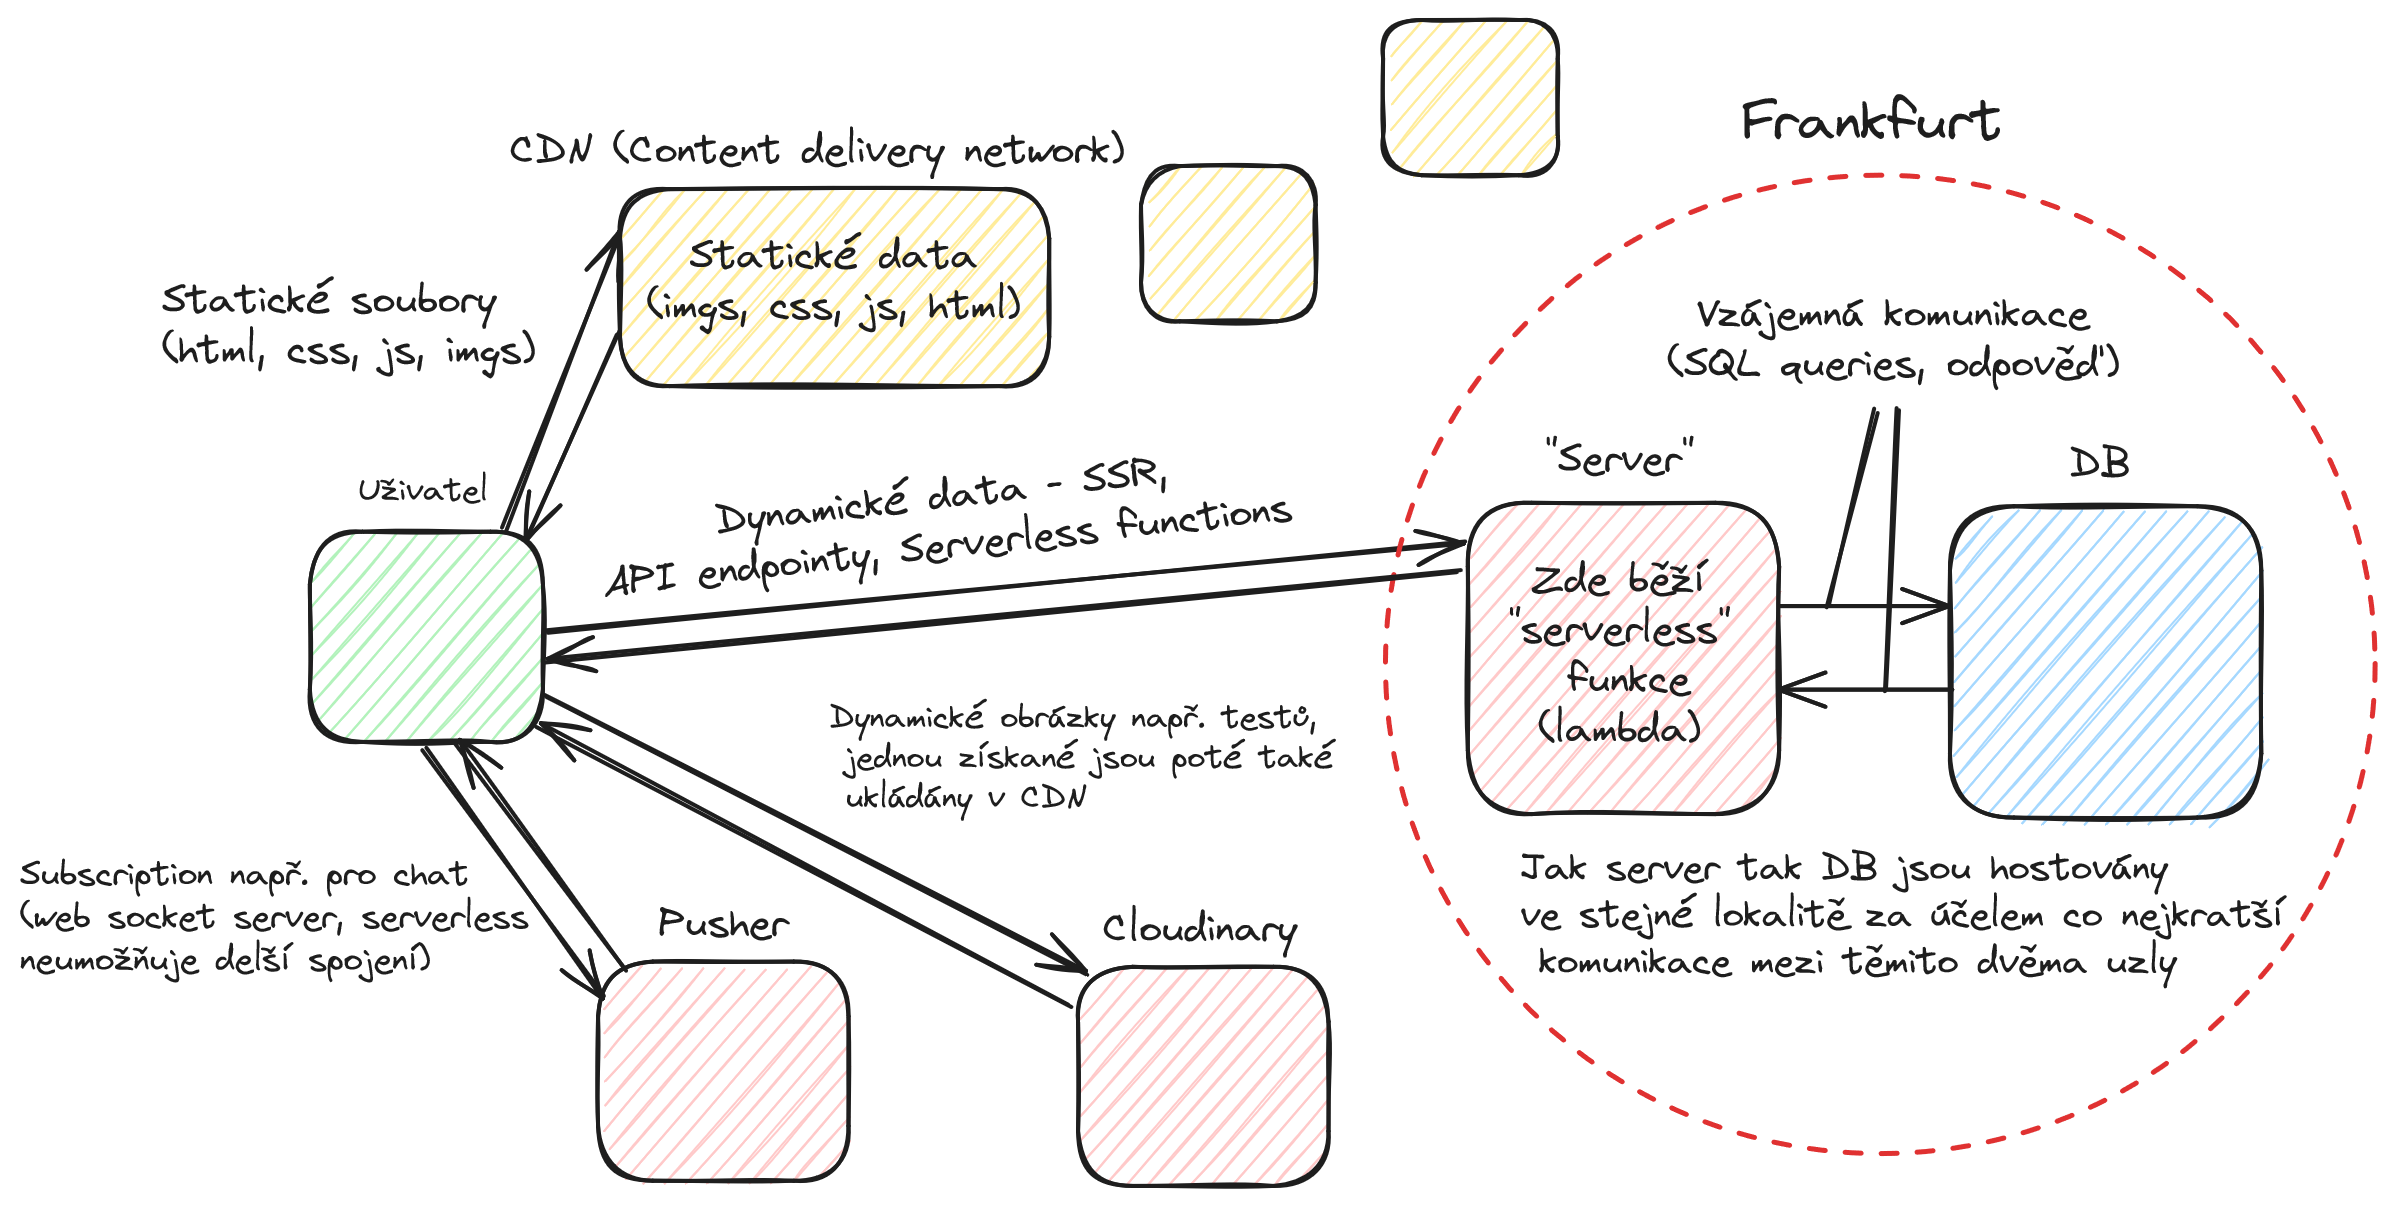
\includegraphics[width=1\linewidth]{image/effio-architecture-simple.png} 
	\caption{Jednoduchý přehled architektury Effia.} %% popisek obrázku, nezapomeň na citace!
	\label{fig:effio-architecture} %% označení až budeš chtít na obrázek odkazovat
\end{figure}

\subsection{Koncept "single page application" a tradičního web serveru }
V minulé sekci jsem zmínil pojem web server, ten generuje stránku, která je poslána uživateli, ta se poté generuje znovu vždy když je uživatel přesměrován na jinout stránku, tento koncept má spoustu nevýhod jako například nemožnost jednoduše uchovávat data mezi těmito přechody."Single page application" je vlastně JavaScript framework, který se o překreslování obrazu a přesměrování stará sám za pomocí JavaScriptu bez nutnosti dotazovat se serveru o novou stránku či data. Tento přístup bohužel také není perfektní, nutnost stahovat veškerý kód nebo velice chabý SEO rating.

\subsection{Metaframework}
Oba zmíněné koncepty přinášejí své výhody ale s ním také nevýhody, Metaframework je technologie, která kombinuje výhody obou konceptů a přináší za mě nejlepší variantu jak vytvářet webovout aplikaci. Disponuje možností běhu kódu na serveru, přesměrováním na klientské části a dalšími výhodami. Takových technologií existuje celá řada, jako například populární NextJS, já si pro svůj projekt zvolil SvelteKit.

\subsection{Cloud hosting}
Jak již bylo zmíněno v~úvodu tak tato aplikace by se měla obejít bez vlastního serveru, nejde ale jenom o databázi ale také například o ukládání obrázků nebo hostování aplikace jako takové, to je prováděno přes "Cloud hostingy" jako Vercel pro hostování stránky jako takové, zároveň ale řeší i rozesílání statických dat do CDN a poskytuje serverless lambda funkce, Cloudinary, který slouží jako "bucket" pro obrázky a také jejich možnost editace přes url parametry, nebo Pusher, který slouží jako web socket server například pro chat.

\section{Typesafety}

Webové aplikace standartně využívají JavaScript, ten ale obnáší signifikantní nevýhodu v podobě nemožnosti "otypovat" kód, to způsobuje obtíž orientovat se v kódu, velké množství produkčních chyb a také spoustu času stráveného pochopením dříve napsaného kódu. Pro Effio jsem se tedy rozhodl využít moderní technologie a vytvořit tak téměř plně "typesafe" (otypovanou) aplikaci. TypeScript v Effiu nahrazuje JavaScript, ten do tohoto jazyka přináší typy. To ale nestačí, API endpointy, stejně jako databázové dotazy stále nemůžou být otypované a proto jsem připojil také knihovny tRPC a Prisma.


\chapter{Využité technologie}

\section{SvelteKit}

Svelte je open source JavaScriptový framework vyvíjený od roku týmem Riche Harrise, jeho hlavní výhodou je rychlost ale také intuitivita, protože jazyk se snaží vypadat jako JavaScript, zatímco rozšiřuje jeho možnosti, díky tomu se za posledních let těší rostoucí popularitě webobých vývojářů. Na rozdíl od ostatních webových frameworků (například React, Angular, Solid nebo Qwik) Svelte disponuje vlastním jazykem, který se zapisuje do \texttt{.svelte} souboru, ten se následně kompiluje do vysoce efektivního JavaScriptu.\\

SvelteKit je metaframework postavený na Svelte. Jeho hlavní výhody se skládají z:
\begin{itemize}
	\item Rychlost - Svelte vytváří velice rychlou aplikaci, v kombinaci s Vitem (bundler) se ale také spojuje s velice rychlým build timem a fast refreshy. To ale není jediné místo kde se rychlost projevuje, za pomocí SvelteKitu se aplikace vyvíjí velmi rychle díky velice malému množství "boilerplate" kódu.
	\item Flexibilita - Aplikace často potřebuje různé typy vykreslování stránek, SvelteKit dovoluje jednoduše nakonfigurovat jednotlivé stránky či cesty pro specifické způsoby jako SPA, SSR, SSG nebo MPA.
	\item Přehlednost - SvelteKit využívá "file based routing", tedy cesty aplikace jsou generovány podle složek, které vývojář vytvoří, soubory se poté vždy jmenují stejně, \texttt{+page.svelte} pro stránku, \texttt{+layout.svelte} pro layout apod. Díky tomu je vždy jasné pro co specifický souboru slouží, přehlednosti také přidává, již u Sveltu zmíněná podobnost s JavaScriptem.
\end{itemize} 

\section{Typescript}
Typescript se dá považovat jako nadstavba JavaScriptu, poskytuje ale jednu výraznou výhodu - typy, díky nim je možno mnohem snadněji dohledávat chyby, vracet se k dříve napsanému kódu a celkově mnohem zlepší "developer experience" při vytváření aplikace. Sám o sobě pomůže s otypováním jednotlivých částí kódu, neporadí si však například s API endpointy nebo databázovými dotazy, které se poté musí otypovat ručně, což je ale velice špatný způsob.

\section{tRPC}
V minulé sekci jsem se zmínil o problémech s otypováním API endpointů, tRPC (Typescript Remote Procedure Call) tento problém řeší tím, že vytváří dynamické typy pro jednotlivé endpointy, podle toho jak si je sami nadefinujeme.

\section{Prisma}
Prisma slouží jako ORM (Object–relational mapping), to znamená pomocí JavaScriptu získávat data z databáze bez přímého použití jazyka SQL, Prisma se skládá z klientské části, která pomocí protokolu založeném na JSON komunikuje se serverovou částí, tam je následně uskutečněn SQL dotaz a odpověď je poslána klientovi. Také řeší již zmíněný problém s otypováním těchto dotazů, pro Prismu je totiž nutné vytvořit \texttt{schema.prisma} soubor kde se definuje model databáze, ten poté můžeme pomocí Prisma CLI nahrávat do databáze ale také vytvářet dynamické typy, které poté využijeme jak v~dotazech tak v~aplikaci pro data, která dostaneme zpět.

\section{Zod}
Zod je validační knihovna jako např. Yup. Jeho výhodou je avšak možnost využít jeho validační schémata jako typy a také samotná validace funguje jako "type guard" (kontroluje a nastavuje typy u vložené proměnné). Jeho další výhodou je například jeho nízká velikost.

\section{Tailwind CSS}
Tailwind CSS je "CSS utility library", to znamená, že narozdíl od frameworků jako je třeba Bootstrap nebo Material UI neposkytuje celé předpřipravené komponenty ale připravené CSS classy, které se aplikují na HTML elementy, jeho výhodou je naprostá kontrola nad chováním stylů, které se aplikují, přehlednost a rychlost se kterou se dá styly vytvářet.

\section{Auth.js}
Auth.js je knihovna sloužící pro autentifikaci a autorizaci, poskytuje možnost "session based", to je použito v Effiu, a JWT autentifikace. Dále knihovna podporuje OAuth s mnohými providery, v tomto projektu je využit GitHub a Google s jednoduchou možností přidat další. Výhodou knihovny je, že data si vývojář spravuje sám, neboli jsou ukládána do jeho vlastní databáze v podobě tabulek (které si také může sám upravit): Account, Session, User a Verification Token, které poskytují naprostou kontrolu nad ověřením uživatelů.

%\section{Cloud provideři}
%Effia plně spoléhá na cloudové řešení, díky nim je jednoduché zprovoznit plně funkční stránku bez jakékoliv starosti o fyzický hardware, stejně jako o škálování zdrojů podle potřeby.
%\begin{itemize}
	%\item \textbf{Vercel} se stará o hostování aplikace jako takové, distribuci statického obsahu na %CDN a jednoduše řeší znovuvytvoření stránky po změně kódu v~GitHub repozitáři. Vercel podporuje %"serverless" architekturu v~podobě tradiční lambda funkcí. Jedná se o instance dané funkce, %která se spouští na serveru, není dedikovaná ale spouští se a vypíná podle vytížení.
%	\item \textbf{Cloudinary} slouží
%\end{itemize}

\chapter{Kroky k řešení, funkcionality aplikace a implementace}
\section{Založení a konfigurace projektu}
Prvním krokem bylo založení projektu a stažení potřebných knihoven technologií, které jsem plánoval využít. Kombinace mnou vybraných technologií nebyla kompletně konvenční a proto jsem se musel v~některých případech obrátit na komunitou vytvořené adaptéry, příkladem je například knihovna \texttt{trpc-sveltekit}, která propojuje SvelteKit a tRPC, které je primárně navrženo buď jako samostatný server a nebo jako implementace do Next.js.

\clearpage
\section{Model databáze}
Dalším krokem bylo vytvořit databázový model, vystavený obrázek nezachycuje model počáteční ale ten, ke kterému postupem práce Effio dospělo přidáváním nových funkcionalit, model byl také několikrát částečně přepracován.
\begin{figure}[H]
	\centering %% příkaz, který ti obrázek zarovná na střed
	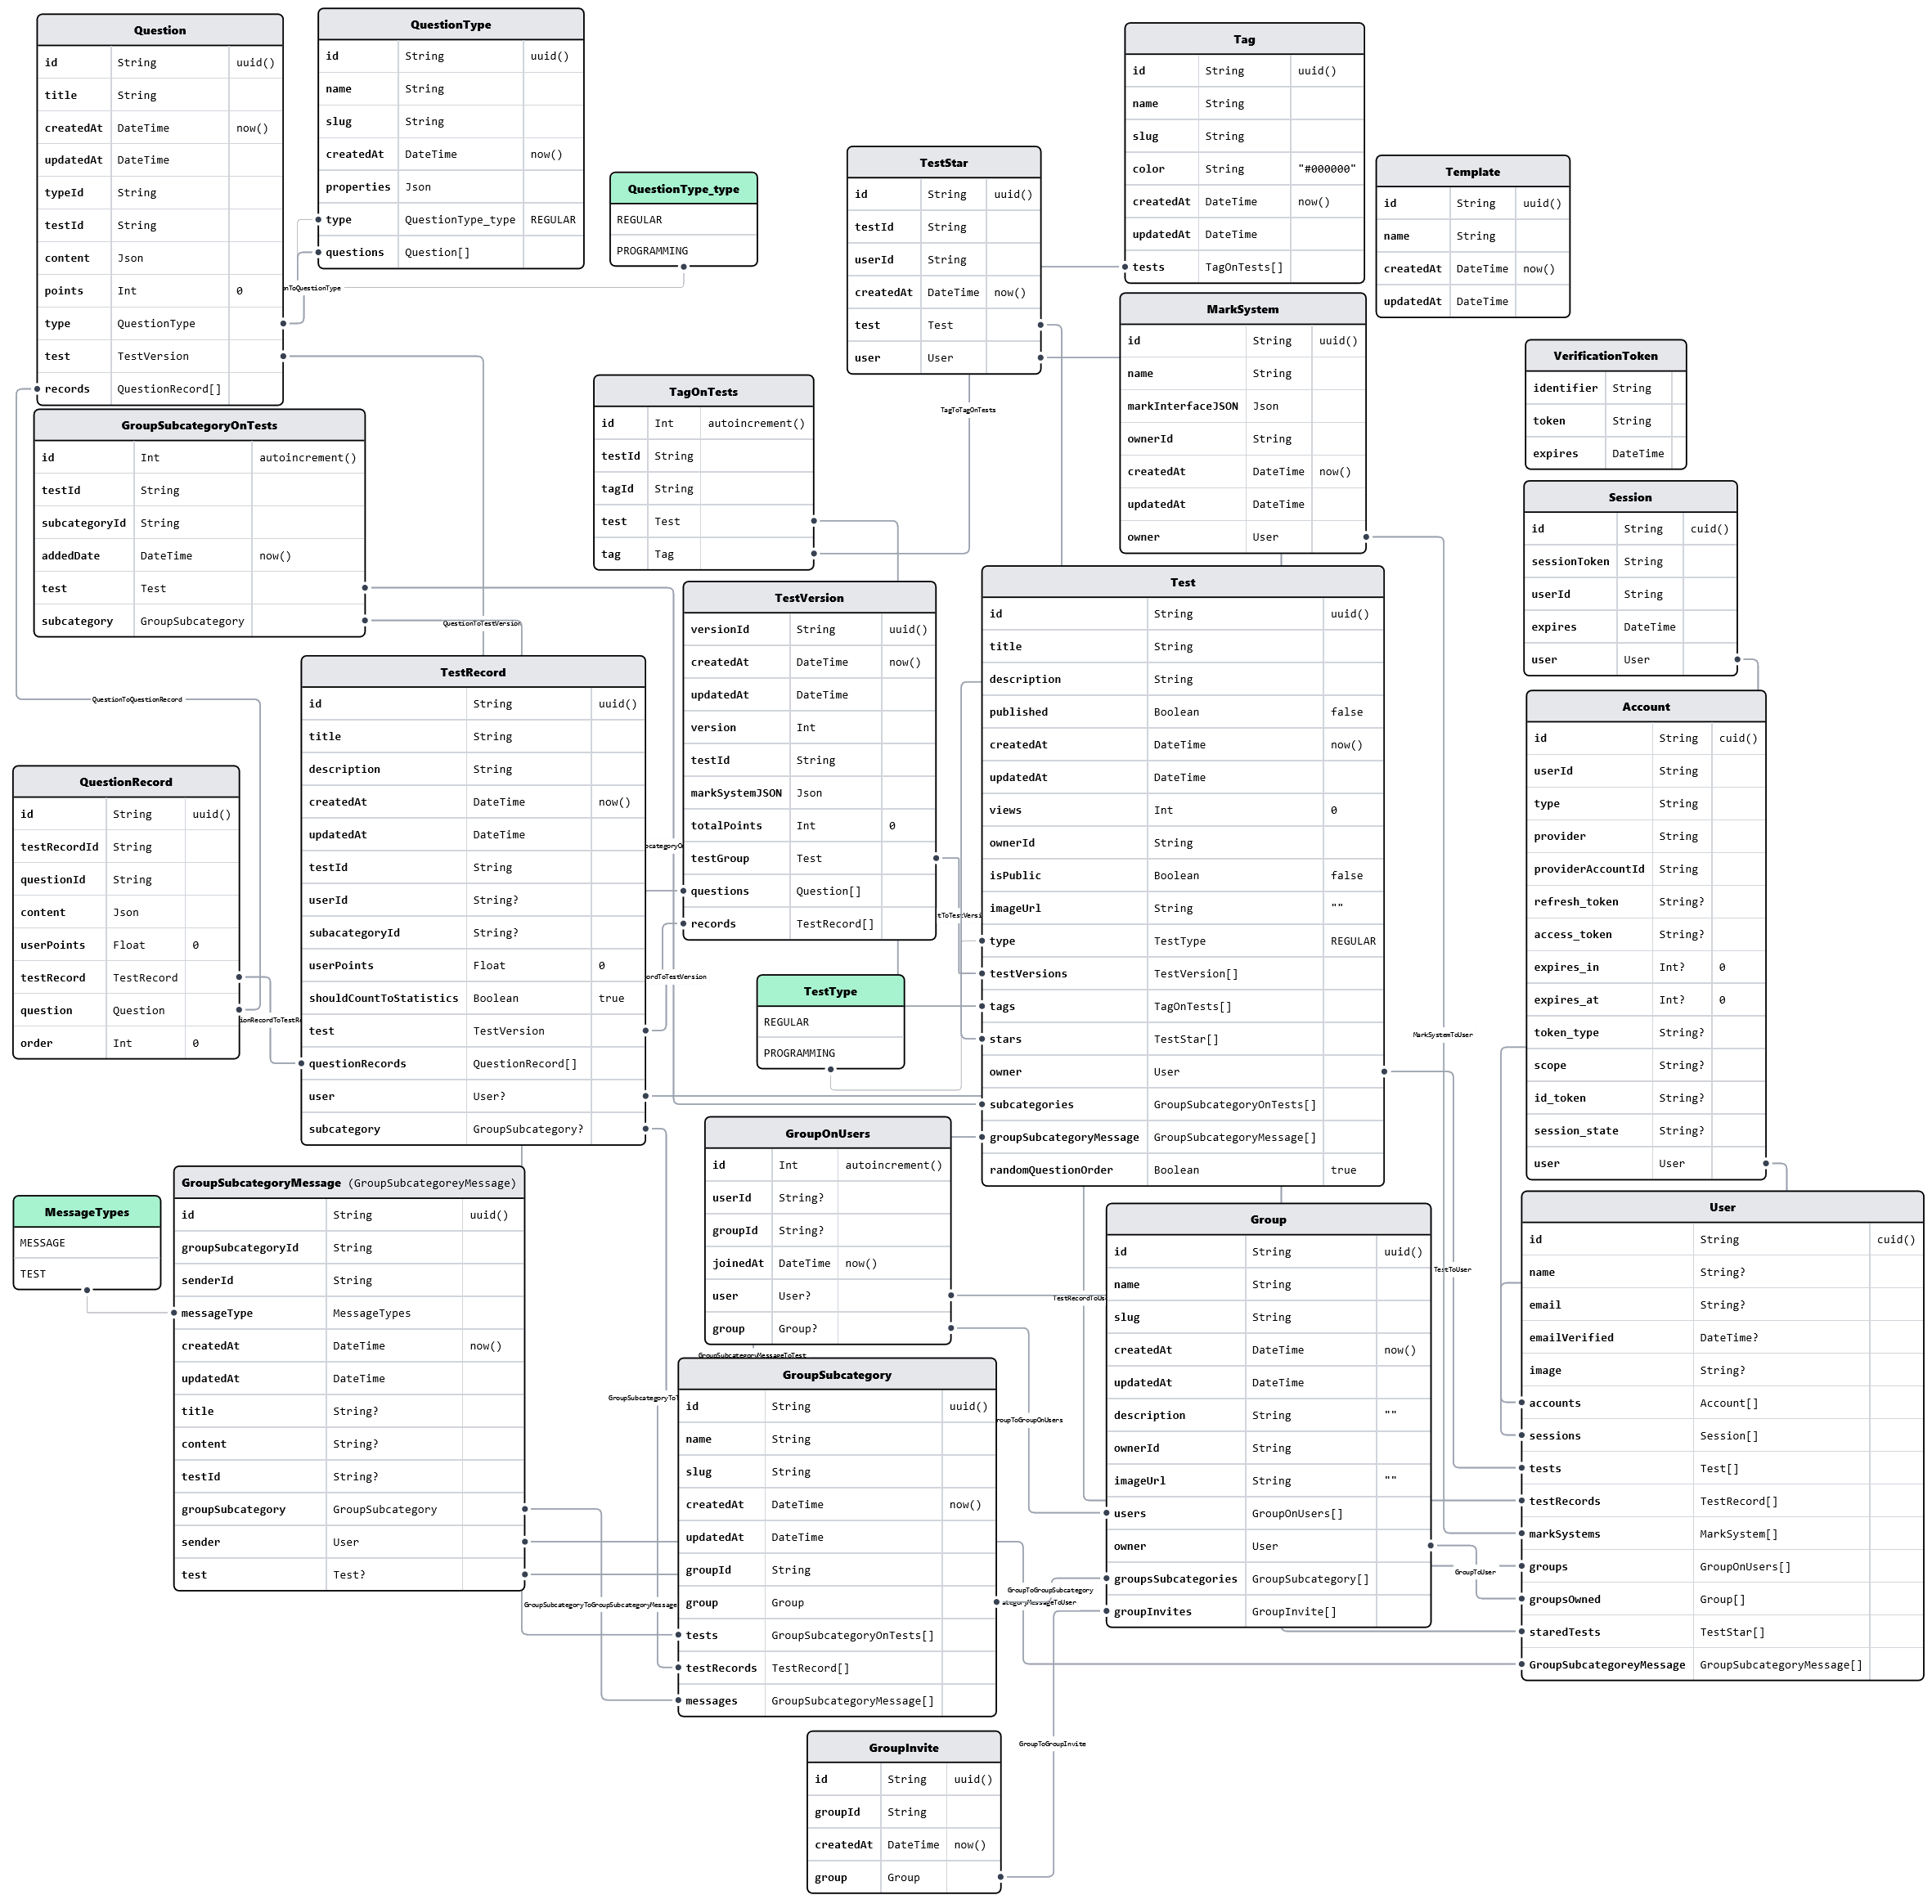
\includegraphics[width=1\linewidth]{image/schema.png} 
	\caption{Databázový model Effia. Vytvořeno pomocí \href{https://github.com/Ovyerus/prismaliser}{Prismaliser}} %% popisek obrázku, nezapomeň na citace!
	\label{fig:schema} %% označení až budeš chtít na obrázek odkazovat
\end{figure}
\clearpage
\section{Design}
Jednou z~hlavních myšlenek bylo vytvořit pohledem přívětivou aplikaci, proto se návrh designu stál klíčovou částí pro stylově propracovanější prvky stránky. Pro tvorbu designu, stejně jako vytváření a úpravu potřebných obrázků jsem využil aplikaci Figma.
\begin{figure}[h]
	\centering %% příkaz, který ti obrázek zarovná na střed
	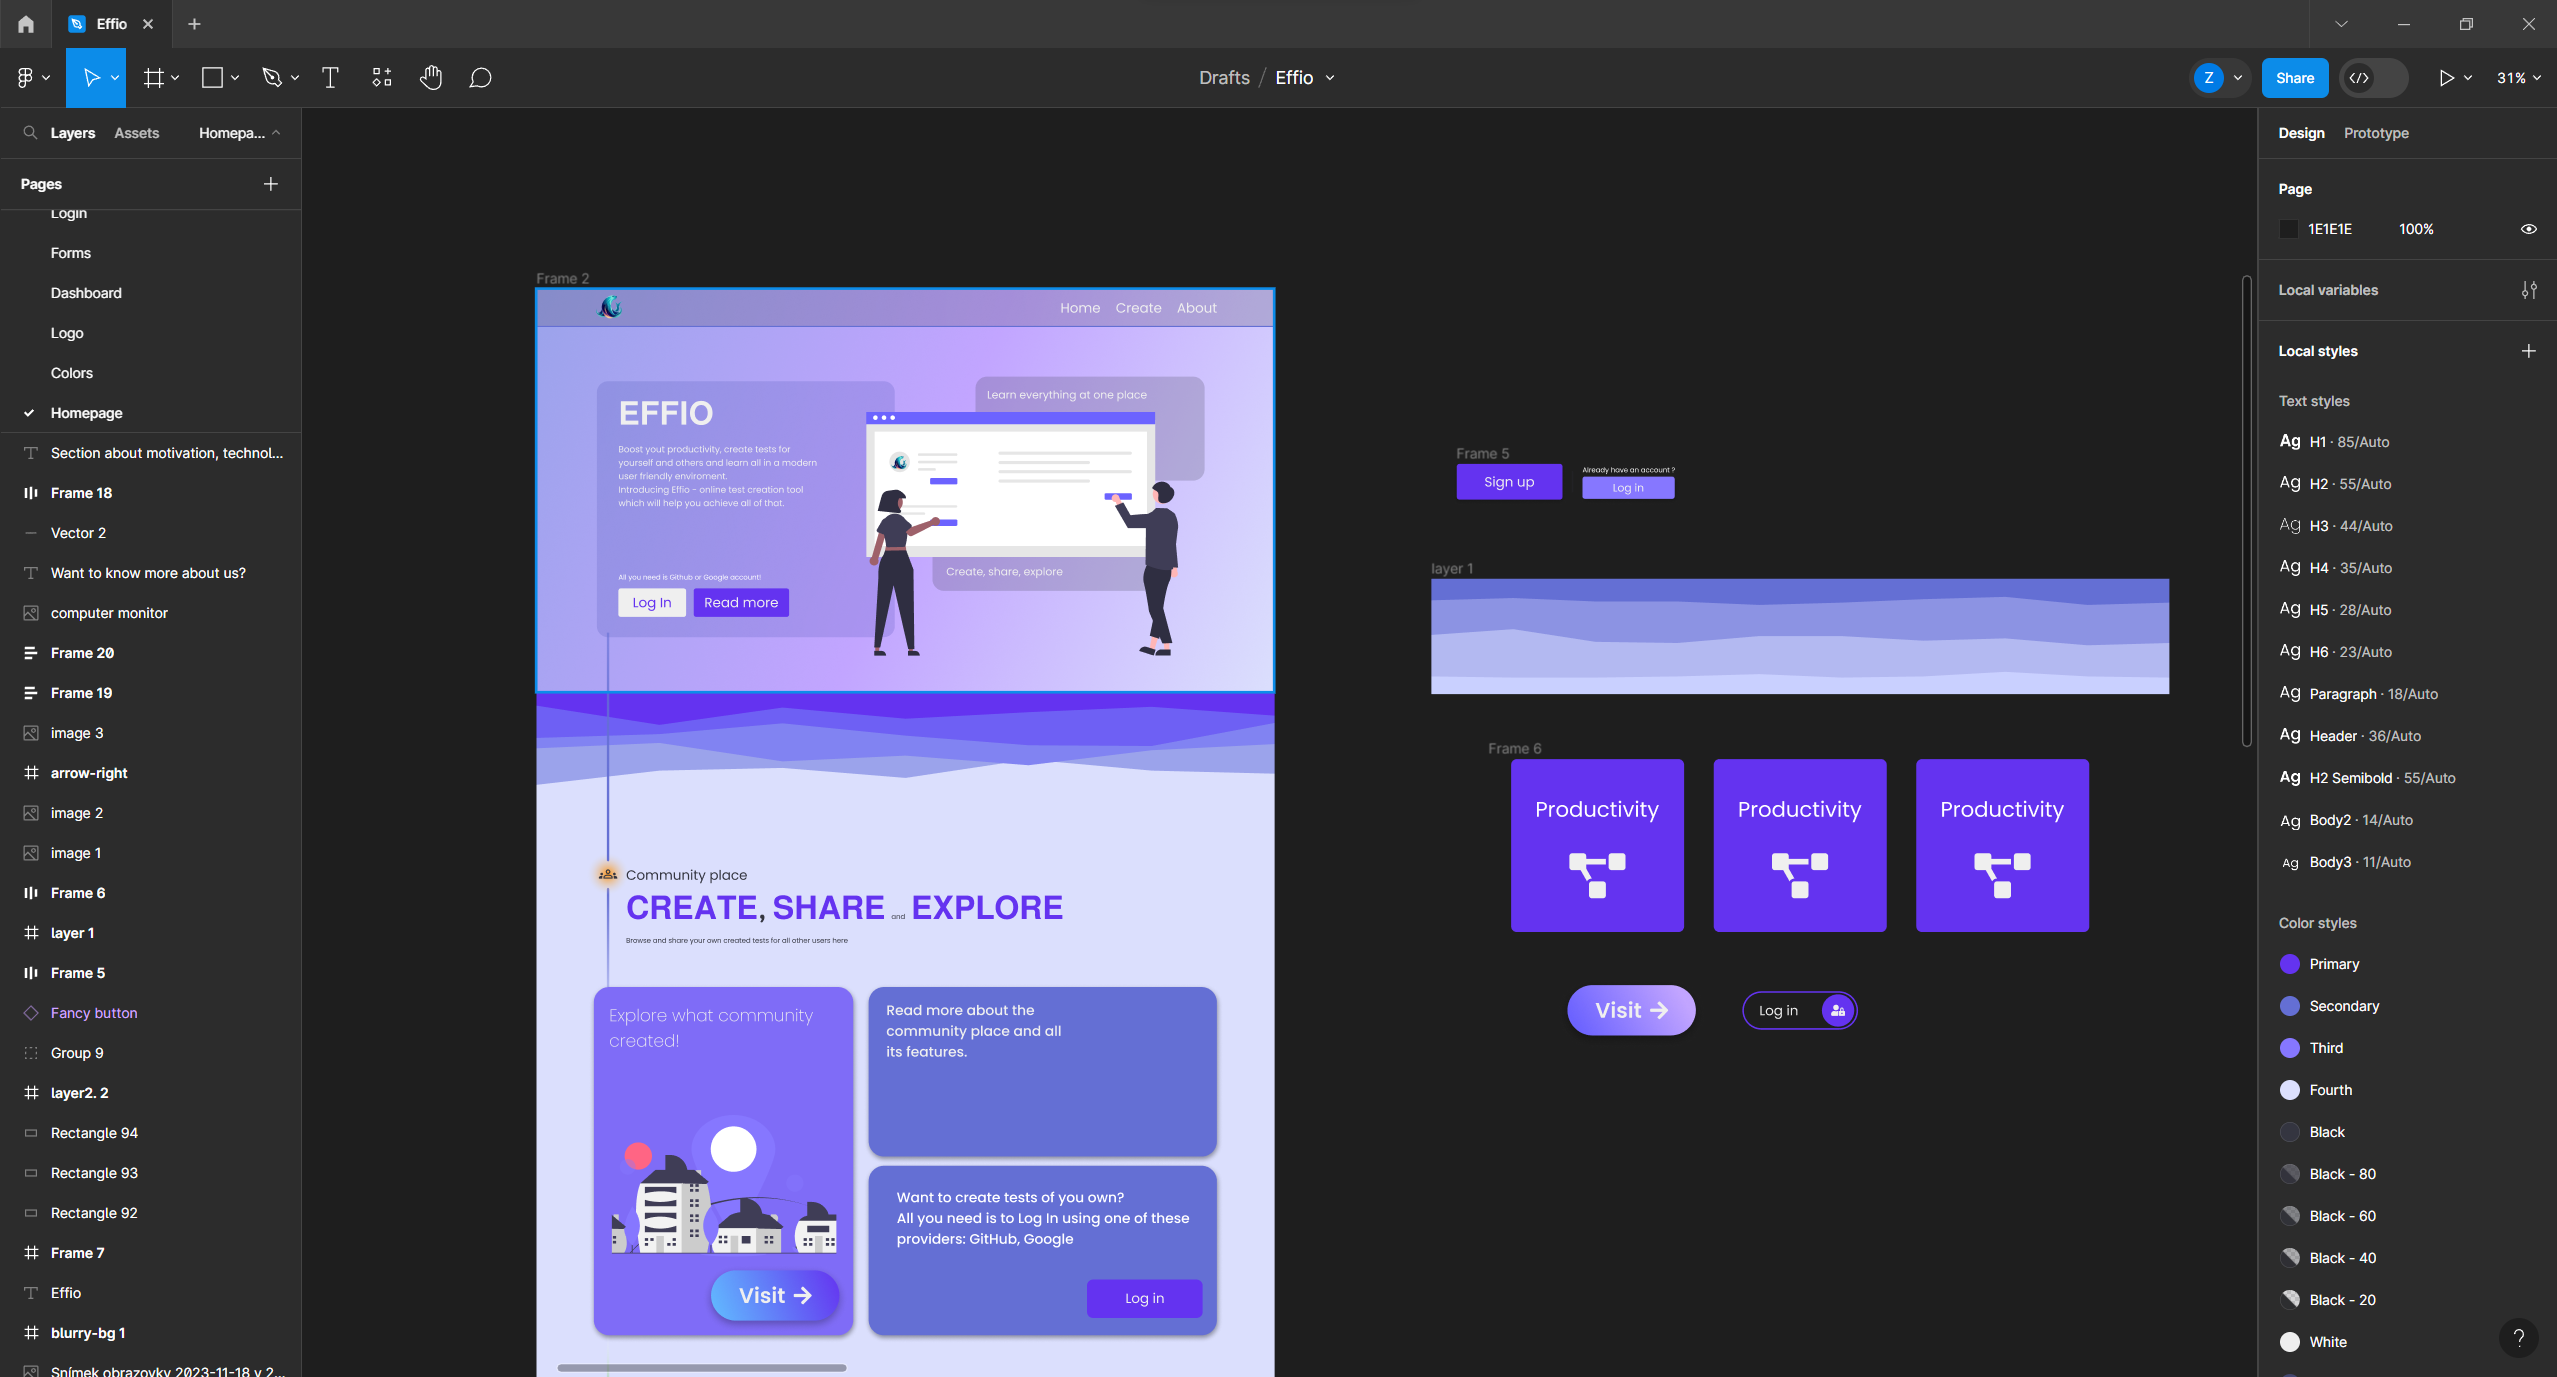
\includegraphics[width=1\linewidth]{image/figma.png} 
	\caption{Prvotní návrh domovské stránky.} %% popisek obrázku, nezapomeň na citace!
	\label{fig:figma} %% označení až budeš chtít na obrázek odkazovat
\end{figure}

\section{Testy a jejich vlastnosti}
Jednou z esenciálních funkcionalit Effia je možnost vytvořit test, k~tomuto existuje mnoho různých postupů, nad danou problematikou jsem se zprvu zamýšlel a až poté napsal funkční nástroj pro jejich vytváření ale to stejně nakonec nezabránilo následné nutnosti přepsat téměř celou funkcionalitu při vytváření testu.

\subsection{Tvorba testu}
\label{subsec:creation}
Jako první si uživatel zvolí mezi kvízovým a programovacím testem, u obou si poté vybere šablonu.
\begin{itemize}
	\item Kvízový - po výběru šablony, kde si uživatel může zvolit i import z GIFT formátu, se uživatel dostane do tvorby testu samotného, vybírat si aktuálně může z~6~typů otázek: \textit{Pick One}, \textit{True/False}, \textit{Connect}, \textit{Write}, \textit{Fill} a \textit{Geography}, otázkám lze svévolně měnit pořadí, přidávat komentáře k~odpovědím a upravovat počet získaných bodů.
	\item Programovací - po výběru šablony se uživatel dostane do tvorby testu programovacího, kde ho pojmenuje problém, popíše co má uživatel řešit, nadefinuje kontrolní vstupy a očekávané výstupy, poté může zanechat nápovědy
\end{itemize}
Po dokončení těchto úprav se uživatel dostane do konečných úprav testu, což činí jméno, popisek a obrázek testu, volitelné zařazení do skupin, tagy, rozhodne se jestli využít známkovací systém, který si může sám upravit, zvolí si zdali náhodně třídit otázky a následně tvorbu ukončí a rozhodne se zdali test uložit jako návrh nebo ho publikovat.

\begin{figure}[h]
	\centering
	\begin{minipage}[]{0.49\textwidth}
		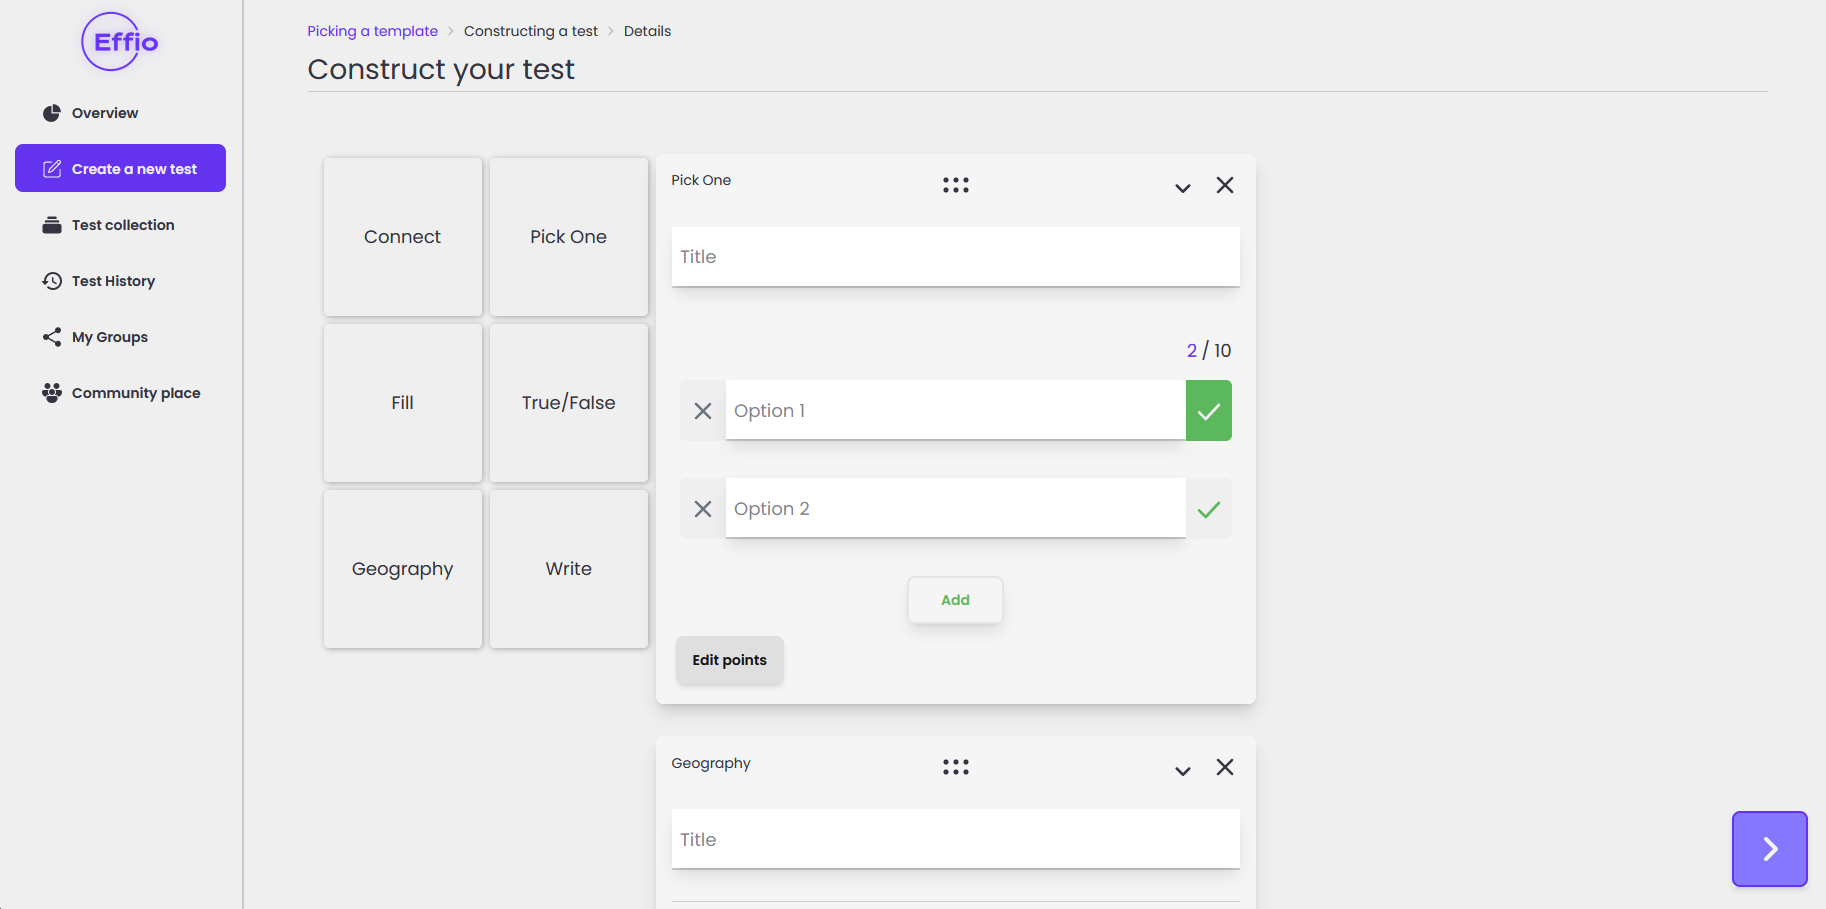
\includegraphics[width=\textwidth]{image/test-creator1.png}
		\caption{Kvízový test}
		\label{fig:test-creator1}
	\end{minipage}
	\hfill
	\begin{minipage}[]{0.49\textwidth}
		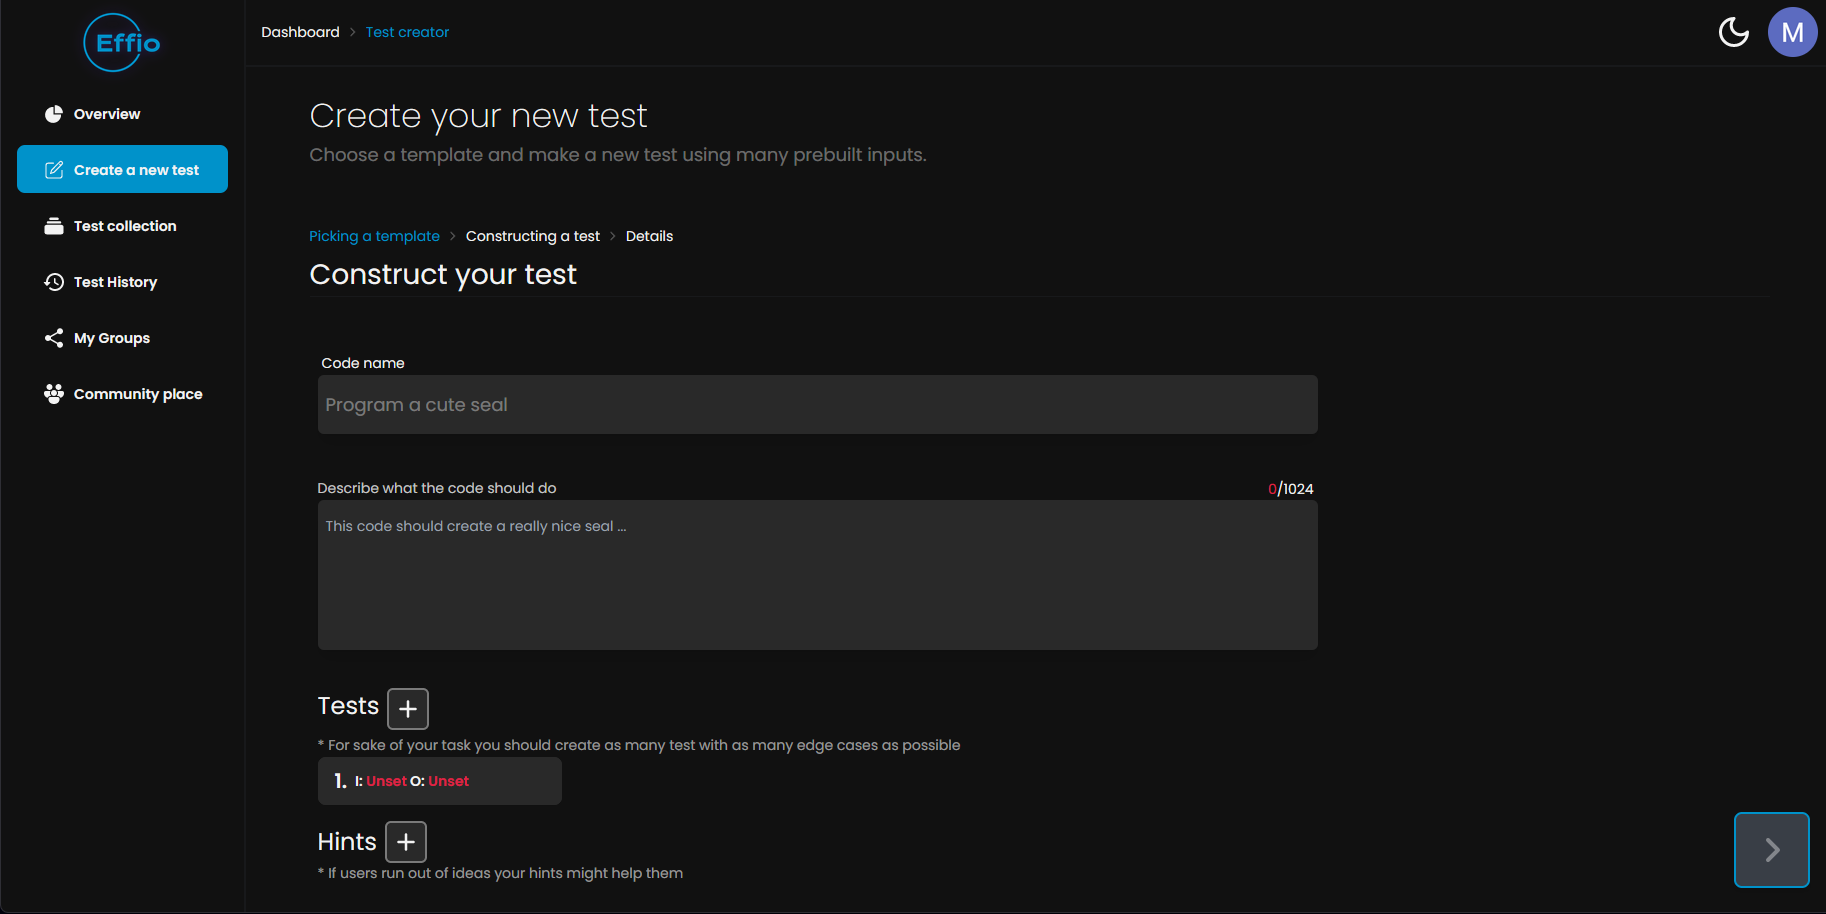
\includegraphics[width=\textwidth]{image/test-creator2.png}
		\caption{Programovací test}
		\label{fig:test-creator2}
	\end{minipage}
\end{figure}

\section{Vyplňování testu}
\label{sec:test-take}
\subsection{Vyplňování kvízu}
Vytvořený test si poté může kdokoliv s~přístupem k~němu vyplnit (testy jsou základně dostupně pro všechny, po úpravě mohou být zveřejněny pouze pro členy skupin).

Otázky se náhodně seřadí a uživatel je vyplňuje, zamíchané jsou také odpovědi určitých typů otázek. Po vyplnění všech uživatel test odevzdá, zkontroluje se a vrátí mu správné odpovědi, počet bodů, známku co získal a pokud je uživatel přihlášený tak se záznam a vyplnění uloží do databáze, uživatel si ho poté může zpětně zobrazit v sekci \textit{Test history}.

\begin{figure}[H]
	\centering %% příkaz, který ti obrázek zarovná na střed
	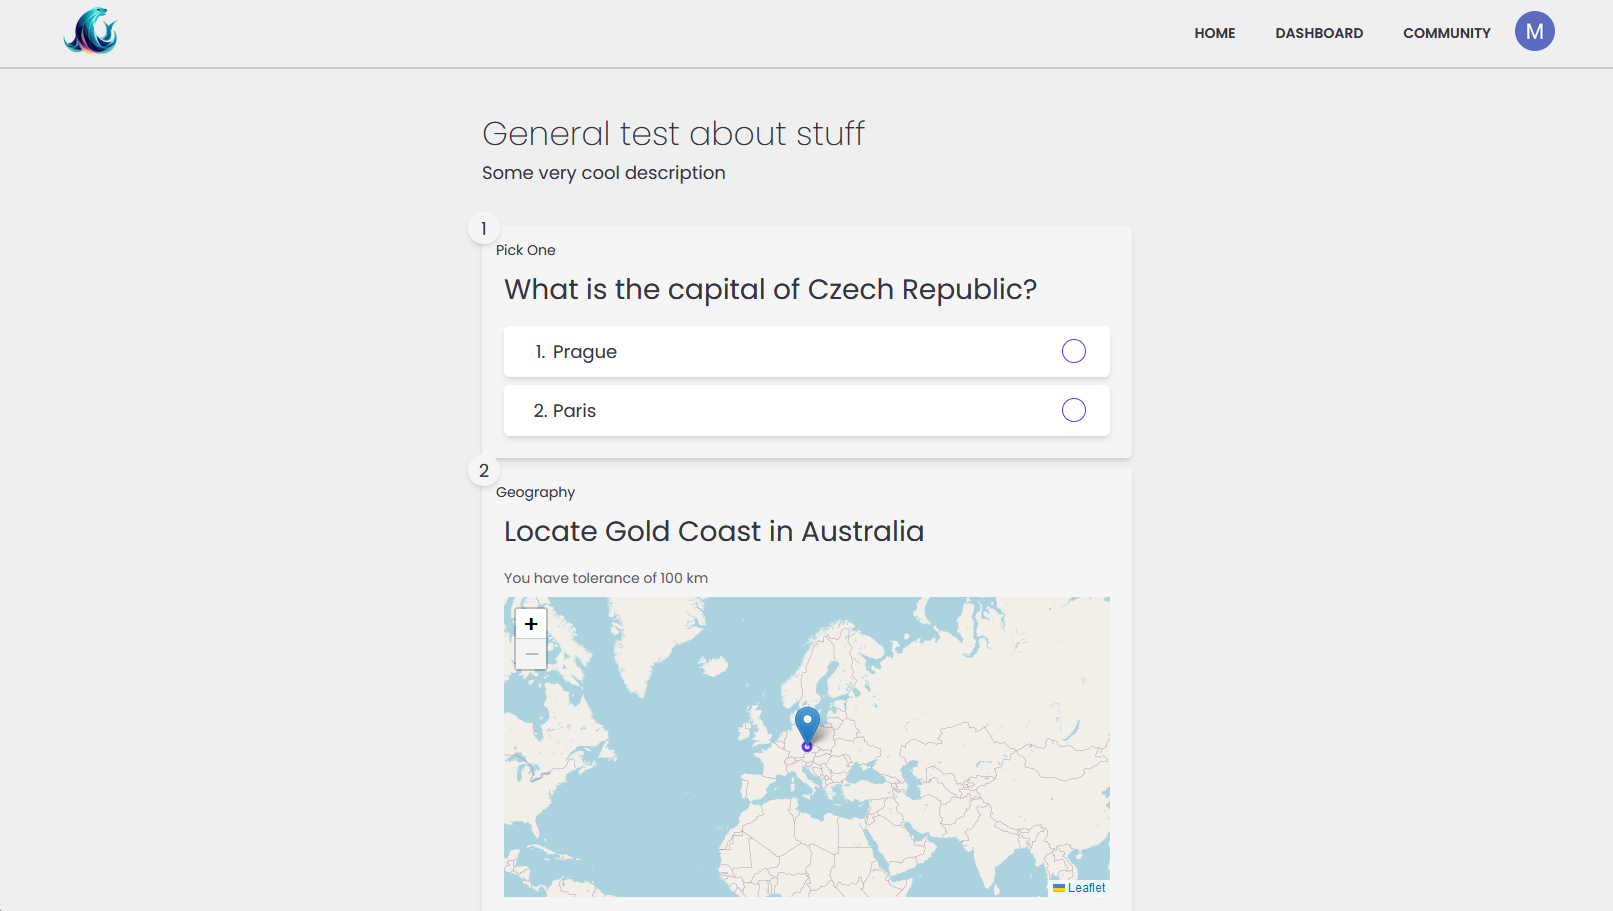
\includegraphics[width=0.75\linewidth]{image/test-taking.png} 
	\caption{Obrázek kvízu.} %% popisek obrázku, nezapomeň na citace!
	\label{fig:test-taking} %% označení až budeš chtít na obrázek odkazovat
\end{figure}

\subsection{Plnění programovacího testu}
Uživatel dostane popis toho co by měl kód umět, sadu testů, které mají otestovat funkcionalitu kódu a popřípadě nějaké nápovědy. Programovací test obsahuje vlastní editor do kterého uživatel píše, pro kontrolu testu můžeme použít tlačítko \textit{"Run"} a pokud testy prochází tak je test možné řešení odevzdat.

\begin{figure}[H]
	\centering %% příkaz, který ti obrázek zarovná na střed
	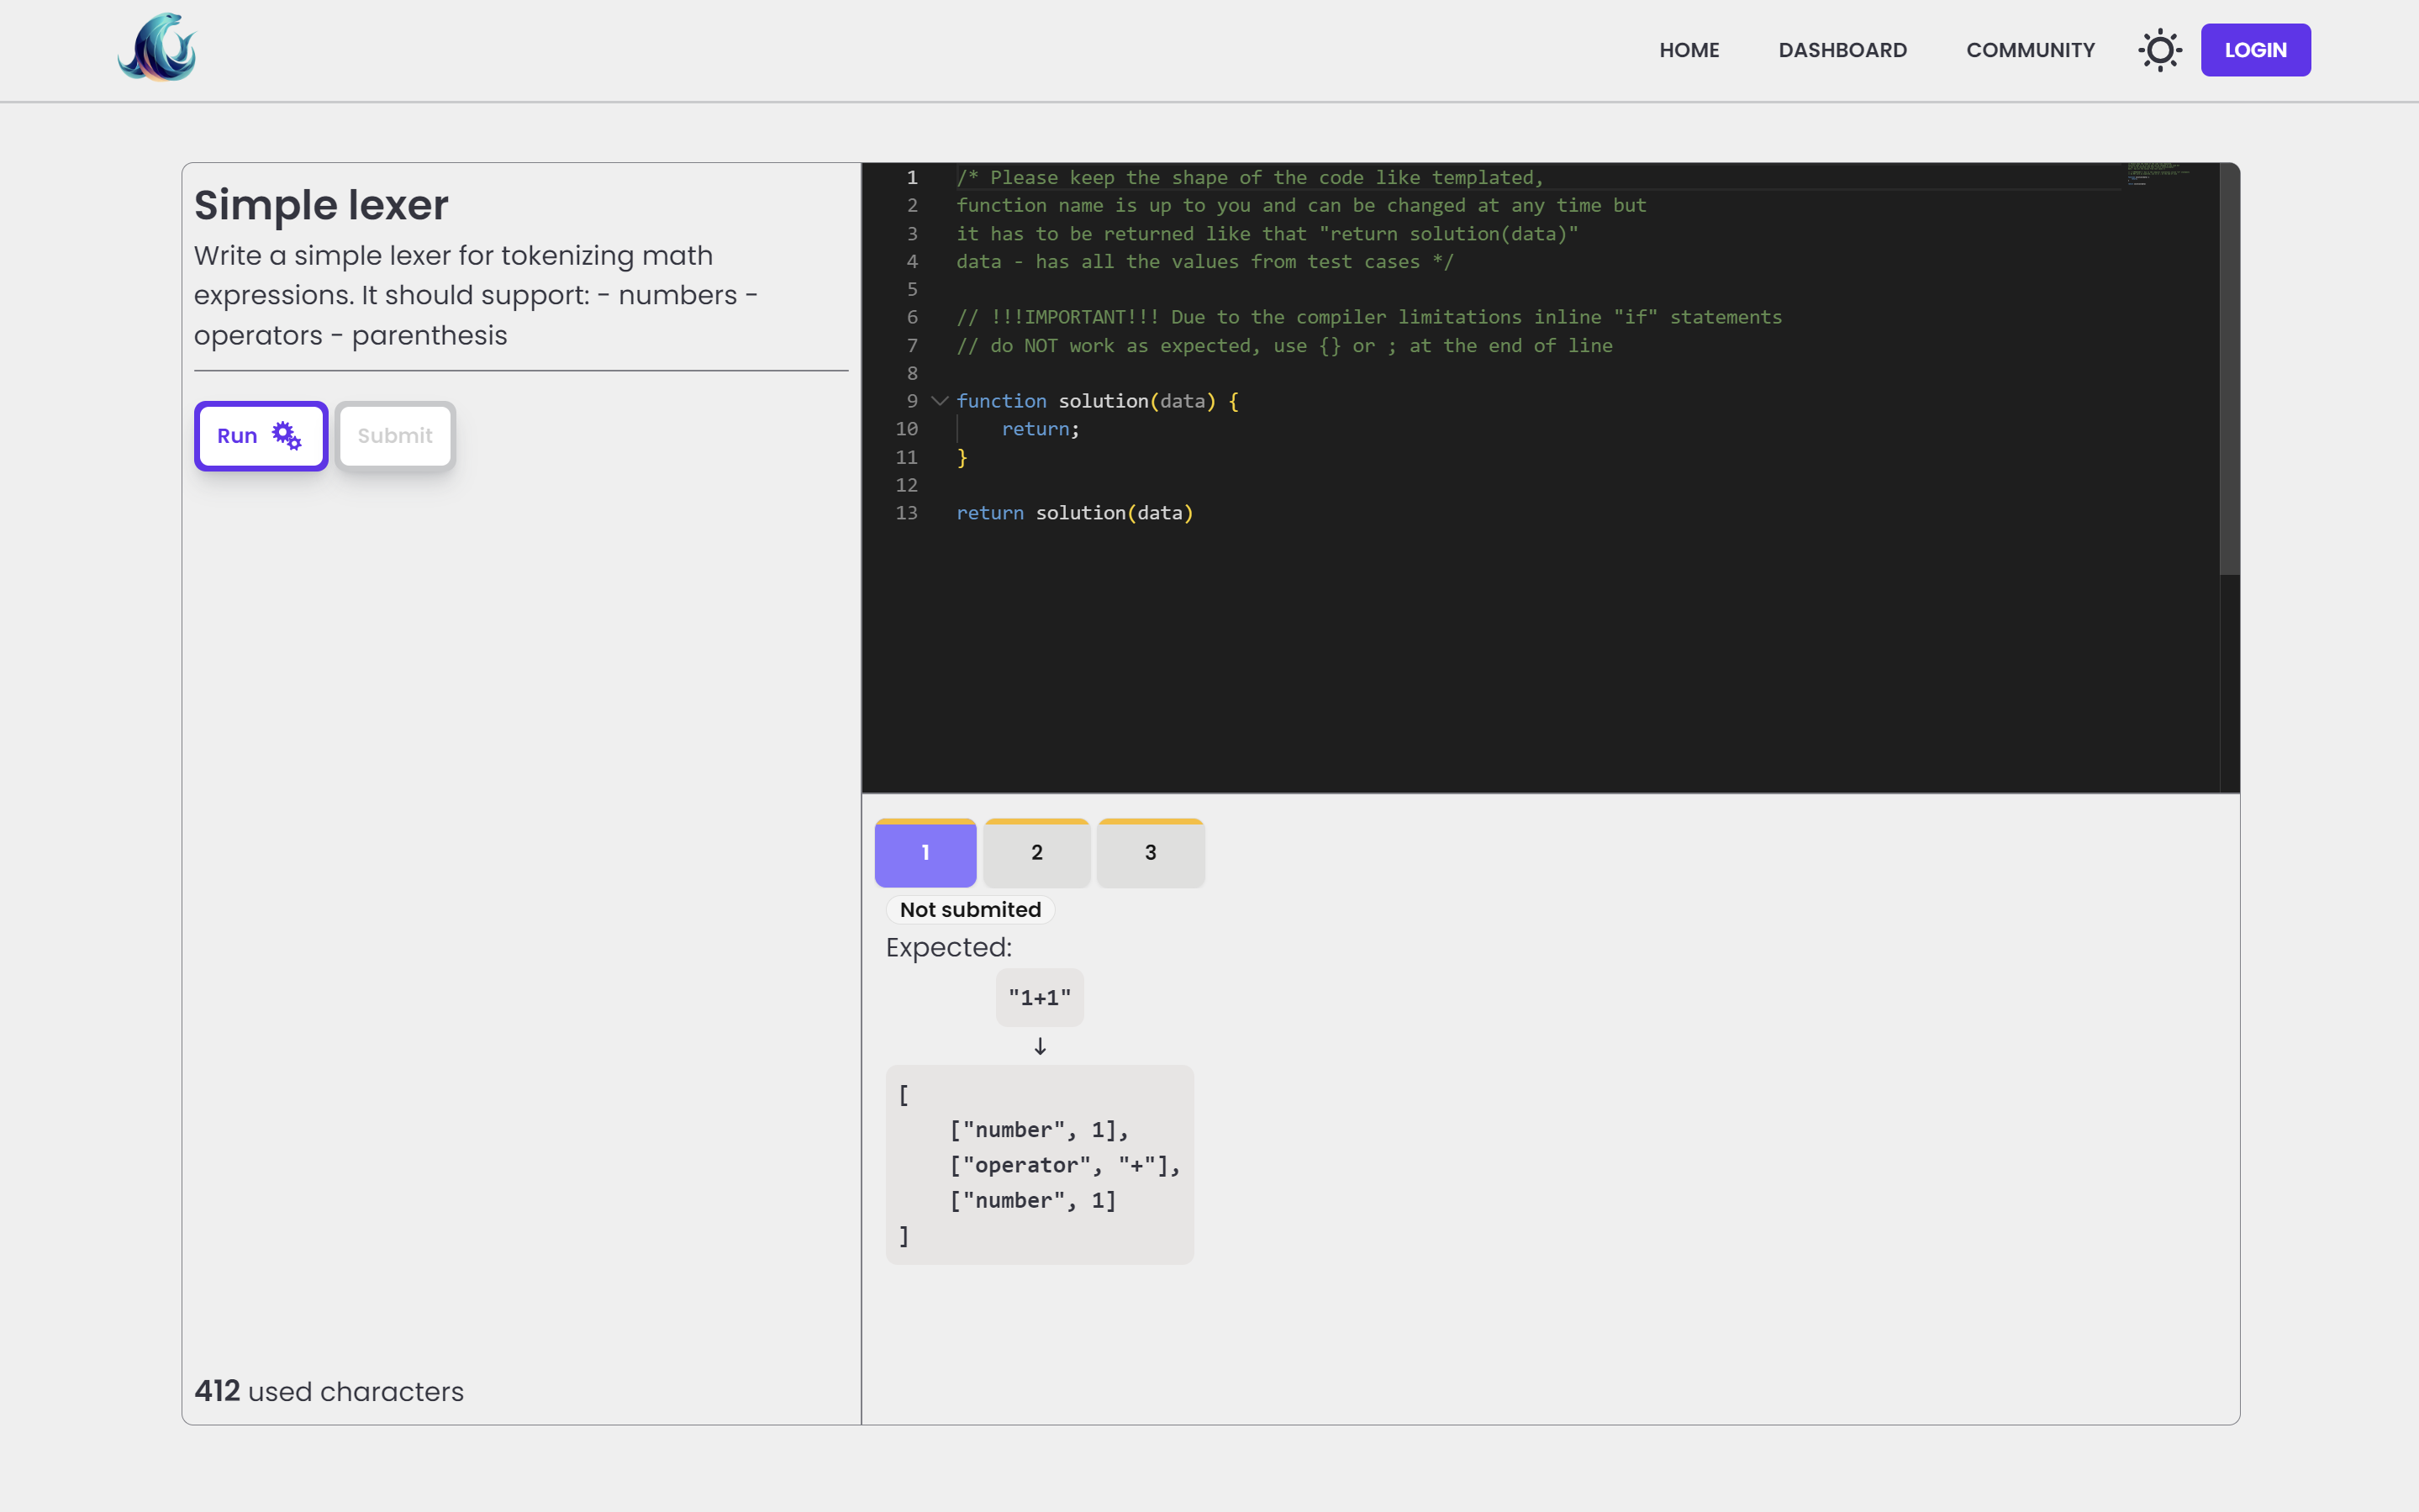
\includegraphics[width=0.75\linewidth]{image/programming.png} 
	\caption{Obrázek programovací úlohy.} %% popisek obrázku, nezapomeň na citace!
	\label{fig:programming} %% označení až budeš chtít na obrázek odkazovat
\end{figure}


\section{Zobrazování testů}

\subsection{Komunitní místo}
\label{subsec:community}
Na této stránce může uživatel najít nové a populární testy včetně všech testů, které existují. Testy jsou zobrazovány postupně podle principu "infinite scrolling", na což využívám JavaScript API Intersection Observer abych zjistil kdy uživatel dosáhl posledního prvku a vyžádal jsem si tak další, implementované je také vyhledávací pole, které filtruje zobrazované testy, další možností je filtrace pomocí tagů. Vizuálně jsou také rozlišeny kvízy od programovacích testů. Testy se také dají ohodnotit hvězdičkou, jejich aplikování využívá principu "optimistic update", to znamená, že po přidání hvězdičky ji uživatel okamžitě vidí přidanou zatímco se ověřuje jeho oprávnění a vytváří záznam hvězdičky v databázi, v~případě neúspěchu se poté uživateli sama hvězdička opět odebere. 

\begin{figure}[H]
	\centering %% příkaz, který ti obrázek zarovná na střed
	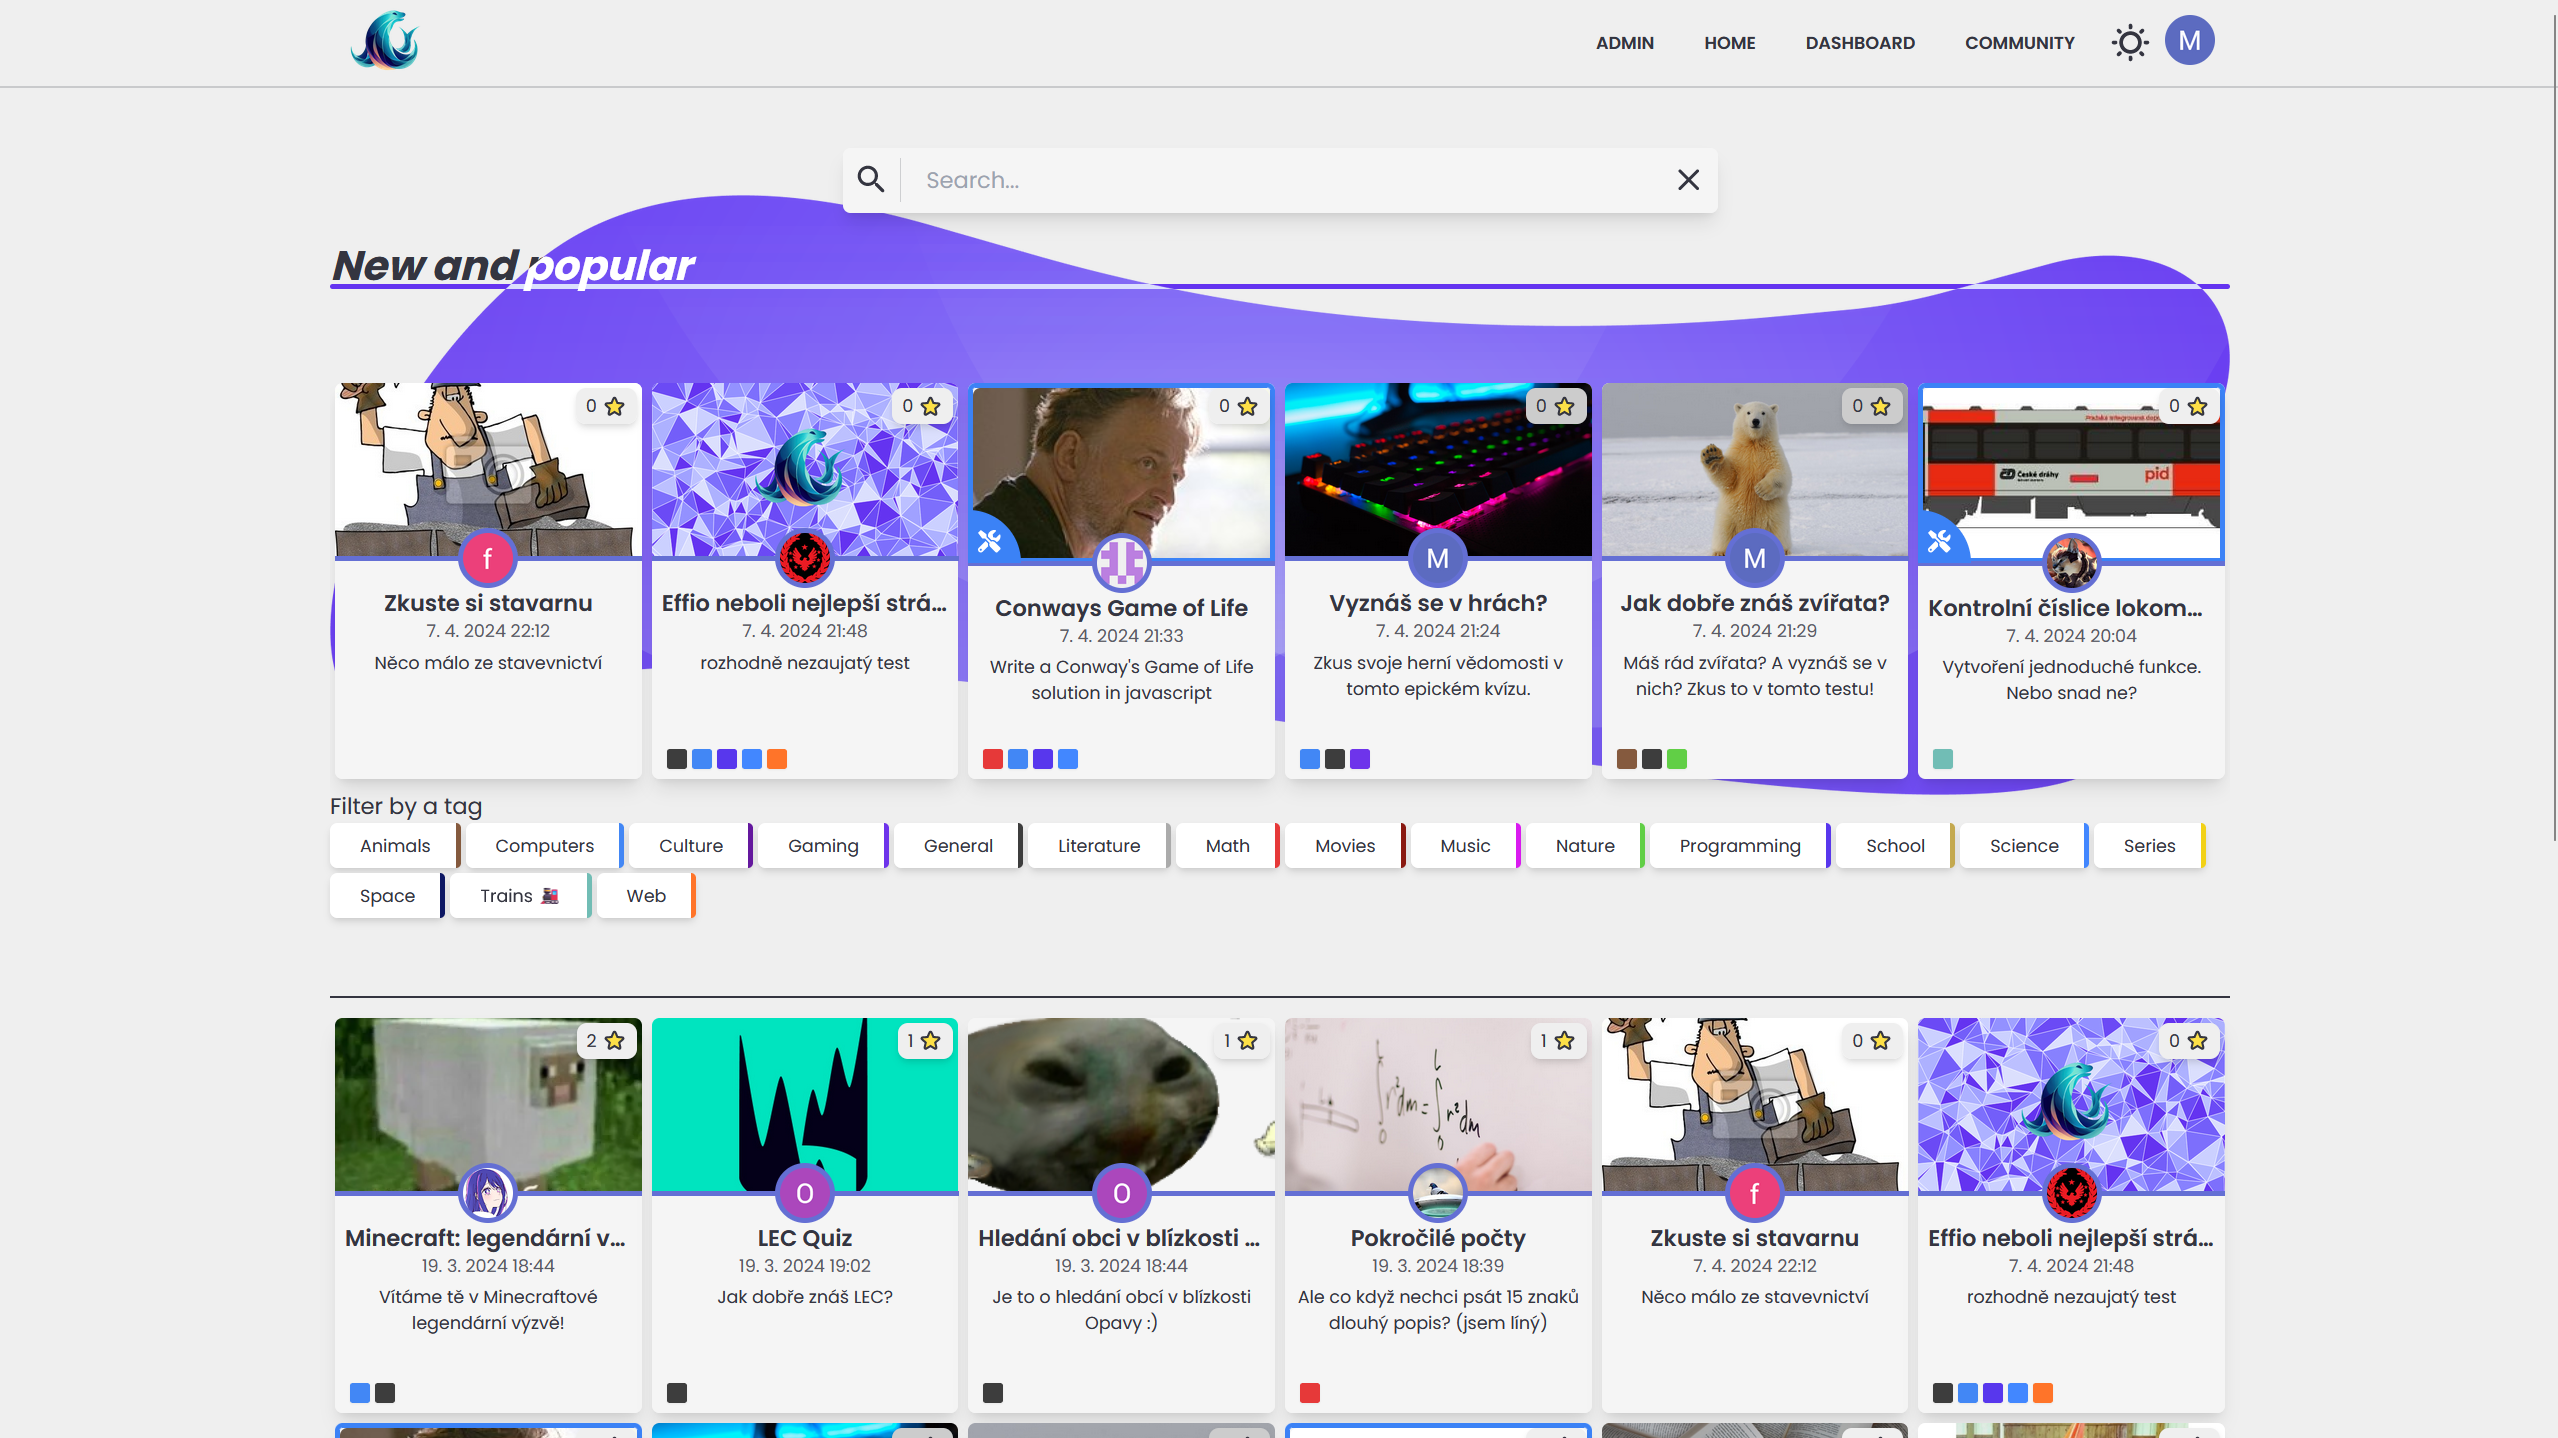
\includegraphics[width=1\linewidth]{image/community.png} 
	\caption{Komunitní místo.} %% popisek obrázku, nezapomeň na citace!
	\label{fig:community} %% označení až budeš chtít na obrázek odkazovat
\end{figure}


\subsection{Kolekce testů}
\label{subsec:collection}
Zde si uživatel může zobrazit jím vytvořené testy, aplikovaná je stejná funkcionalita vyhledávacího pole a "infinite scrollingu". Každý test má ale také další možnosti, a to úpravu, export a smazání.
\begin{itemize}
	\item Úprava - uživatel se přesune na stránku úprav, tam může celý test přepracovat.
	\item Export - vytvoří z~testu textový soubor ve formátu GIFT se všemi otázkami daného testu, které jsou podporovány Moodlem
	\item Delete - smazání testu z databáze
\end{itemize}


\section{Skupiny}
Každý přihlášený uživatel si může vytvořit vlastní skupinu, do které se můžou pomocí generovaného kódu připojit ostatní uživatelé. Skupina obsahuje kanály, ve kterých je možné psát textové zprávy, taky zde můžeme nají přidané testy, vlastník si poté může procházet grafy výsledku členů skupiny.


\section{Světlý a tmavý režim}
S ohledem na uživatele co preferují tmavý režim jsem se také rozhodl pro tvorbu tmavého režimu, ten je možné vidět na obrázku \ref{fig:test-creator2}, oba tyto režimy vyžadovali vlastní paletu barev a byly mnohokrát přepracovány aby k~sobě jednotlivé barvy co nejlépe pasovaly.

\section{Domovská stránka}
Domovská stránka slouží jako místo pro seznámení návštěvníka s~výhodami Effia, rychlá navigace mezi jednotlivými stránkami ale také jako místo nejpečlivěji vytvářeného designu a efektů aby na uživateli zanechala dojem kvalitní aplikace.

\begin{figure}[h]
	\centering %% příkaz, který ti obrázek zarovná na střed
	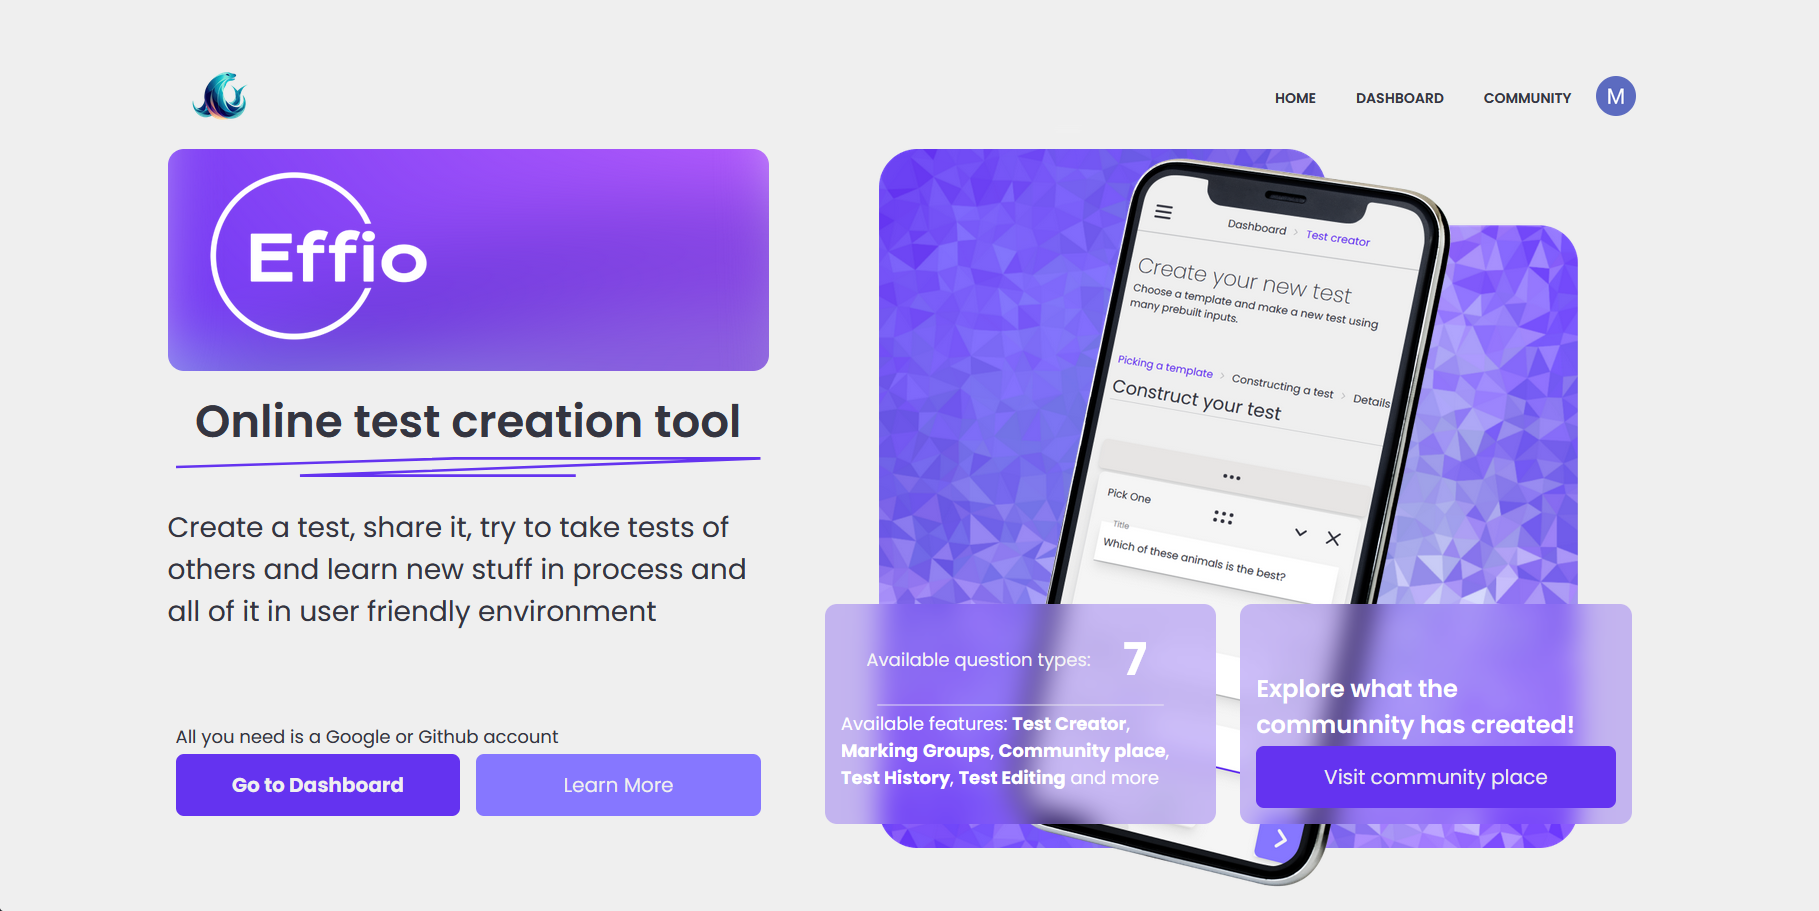
\includegraphics[width=1\linewidth]{image/homepage.png} 
	\caption{Domovská stránka Effia.} %% popisek obrázku, nezapomeň na citace!
	\label{fig:homepage} %% označení až budeš chtít na obrázek odkazovat
\end{figure}
\clearpage
\section{Responsivita}
Celá aplikace je uzpůsobená jak pro počítače tak pro mobilní zařízení. Responsivita není vůbec lehká práce, mně ale pomohl Tailwind, ve kterém se CSS media query dělají snadněji společně s moderními CSS containers, které umožňují responsivní breakpointy odvozovat ne jen od velikosti stránky ale od rozměrů rodičovských elementů.

\begin{figure}[h]
	\centering
	\begin{minipage}[]{0.49\textwidth}
		\centering
		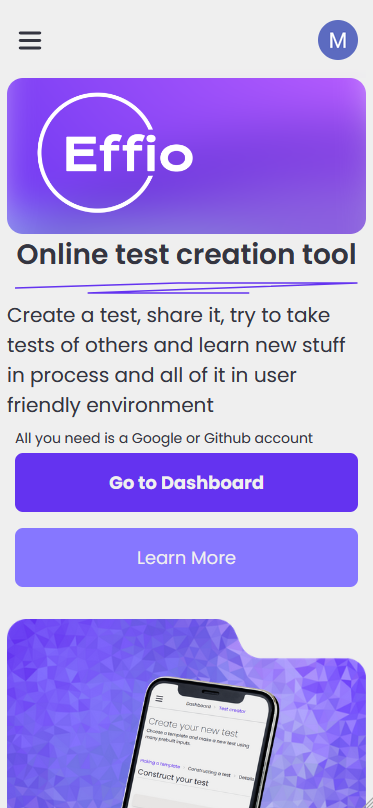
\includegraphics[width=0.5\linewidth]{image/res1.png}
		\caption{Domovská stránka na mobilním zařízení}
		\label{fig:res1}
	\end{minipage}
	\hfill
	\begin{minipage}[]{0.49\textwidth}
		\centering
		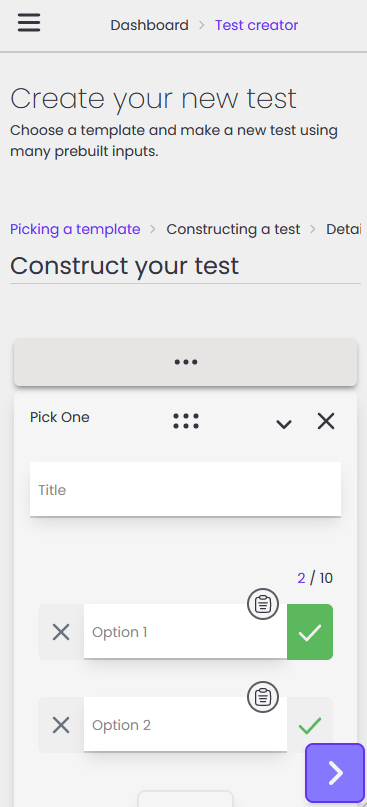
\includegraphics[width=0.5\linewidth]{image/res2.png}
		\caption{Generátor testů na mobilním zařízení}
		\label{fig:res2}
	\end{minipage}
\end{figure}

\chapter{Výsledky práce}
\section{Funkce aplikace}
Po příchodu na stránku se uživateli zobrazí domovská stránka, zde může prozkoumat výhody aplikace nebo se přihlásit, to ho přesune na přihlašovací stránku, na ni se uživatel do aplikace může přihlásit pomocí Google nebo GitHub účtu. Po přihlášení je uživatel přesunut na dashboard, kde může vidět rychlou navigaci na další části nebo se podívat na souhrn jeho aktivity v~grafech. První možností je vytvořit si nový test, tato možnost je detailně probraná zde \ref{subsec:creation}.
Po vytvoření testu je přesunut do kolekce jeho testů, kde může své testy procházet a upravovat, více popsáno zde \ref{subsec:collection}. Test si poté může uživatel zkusit vyplnit \ref{sec:test-take}, buď přímo ze své kolekce nebo z komunitního centra \ref{subsec:community}, kde může najít také testy jiných. Po dokončení testu se dozví výsledky, ty může poté najít zpětně v~sekci \textit{Test history}, kde jsou uspořádané v tabulce.

\section{Splněné a nesplněné cíle}
Cíle byly rozdělené jak do rozsahu aplikace tak do kvality implementace jednotlivých prvků, co se týče rozsahu tak ten jsem v~určitých místech významně předčil, ne všechny body původních cílů jsou ale aktuálně plně dosaženy.

Hlavním cílem bylo vytvořit rychlou, cloudovou aplikaci pro vytváření a sdílení testů využívající moderních "techstack", v~tomto ohledu jsem cíl kompletně splnil, aplikace je v~těchto bodech plně funkční a můj původní plán využití technologií se během vývoje ještě významně rozrostl.

Za úspěch považuji také grafickou část aplikace, která za mě tvoří minimalistický moderní vzhled.

Hlavní neúspěch nebo spíše nedodělanost vidím ve skupinách a přizpůsobení možností testů pro ně, původně jsem zamýšlel vytvořit skupiny jako místo pro sdílení materiálů s více zajímavými možnostmi pro vlastníka, aby sloužili jako funkce vhodná pro výuku. Cíle nejsou zdaleka nerealistické ale těchto cílů jsem nebyl schopen dosáhnou z~nedostatku času, jako vylepšení by ale za mně bylo velice přínosné.

	\chapter{Tipy k psaní}
	\pagestyle{fancy}
	Jak už jsem psal výše \LaTeX je dosti komplexní systém, který umožňuje psát velmi rozsáhlé text. Jeho autor Donald Knuth ho stvořil, aby mohl vydat jeho učebnici \emph{The Art of Computer Programming} a dodnes se je využíván pro sazbu skript, učebnic, článků či závěrečných prací. V této kapitole najdeš ukázky různých funkcí a balíčků \LaTeX u od těch nejzákladnějších až po složitější. Neznamená to nutně, že všechny musíš použít, ale když potřebuješ pomoct, tak je dobré mít oporu. 
	
	Pokud s \LaTeX em úplně začínáš tak ti můžu doporučit přiručku \emph{Ne příliš stručný úvod do systému \LaTeX2e}~\cite{LaTeXprirucka}. Případně spoustu užitečných informací nalezneš na Wikibooks~\cite{wikibooksLaTeX}. Pokud narazíš na nějaký problém googli. Na internetu je spoustu fór, kde pravděpodobně už někdo podobný problém řešil. Asi nejvíce otho najdeš na stránce \emph{TeX - LaTeX Stackexchange} \cite{stackExchange}.
	
	
	\section[Základy]{Základy: Text, obrázky, tabulky a citace} %%[Text, který bude v obsahu]{Text, který se vytiskne na stránce} Zkus měnit jednotlivé závorky a uvidíš :) 
	Psaní v \LaTeX{u} není žádná věda, stačí psát normálně do zdrojového souboru. Pokud bys chtěl psát obrážky či číslovaný seznam, pak můžeš použít prostředí \texttt{itemize} či \texttt{enumerate}. Často je důležité používat nezlomitelnou mezeru. Tu uděláš pomocí \verb|~|~(tildy). Pokud budeš chtít psát uvozovky použij příkaz \texttt{uv}, pomocí něj se ti vytvoří uvozovky podle příslušného jazyka. V česku tedy ve formátu 99 66. Použití příkazu najdeš níže v textu.
	
	Občas je zapotřebí \LaTeX{u} pomoct při rozdělování slov. To se udělá snadno vložením symbolů \verb|\-| mezi jednotlivé slabiky.
	
	\subsection{Tabulky}
	
	U tabulek platí to stejné co u obrázků. Zarovnávají se na střed a nechávají se \uv{plavat} v textu. Tabulka narozdíl od textu, má popisek nahoře. U tabulky \ref{tab:ukazka} je použit balíček \texttt{booktabs}, pomocí kterého je celá tabulka naformátovaná.
	
	Seznam jak obrázků tak tabulek je pak vytvořen pomocí příkazů \texttt{listoftables} a~\texttt{list\-of\-fig\-ures} na konci práce před literaturou.
	
	\begin{table}[h]
		\caption{Tato tabulka slouží jako ukázka toho, jak mohou tabulky vypadat.} %% popisek se u tebaluky píše nad ní
		\label{tab:ukazka} %% označení pro pozdější odkazování se 
		\centering
		\begin{tabular}{lll}
			\toprule %% příkazy z balíčku booktabs
			záhlaví& této & tabulky\\
			\midrule
			obsah&tabulky& už\\
			není & oddělený &čarami\\
			\bottomrule
		\end{tabular}
	\end{table}
	
	
	\subsection{Obrázky}
	
	U obrázků je dobré používat vektorové formáty, pokud to jde. \LaTeX se nejvíc kamarádí s formátem PDF. Do známého PDFka lze z jiných vektorových formátů (ať už SVG či ESP) obrázky přenést snadno pomocí grafických programů, jako je třeba Inkscape. \LaTeX si rozhodně poradí i s tradičními formáty PNG a JPG, avšak tyto obrázky mohou zabírat více prostoru a při tisku se může projevit nižší rozlišení obrázků. Pokud chceš používat tyto obrázky, rozhodně měj na paměti, aby měli rozlišení alespoň 250 indálně 330 ppi.
	
	Obrázky se vkládají do prostředí \texttt{figure}, při úpravě šířky je možné krom tradičních jednotek jako cm nebo mm použít také jako jednotku šířku stránky \texttt{textwidth} to se hodí zejména když chceš mít více podobrázků. 
	
	U každého obrázku je důležité aby měl popisek, \texttt{caption}. Do popisku napiš, co na obrázku je, případně nějaký další popis, tak aby čtenář následně neměl sebemenší pochybnost. U obrázků co nejsou tvoje nezapomeň an citaci. Jinak by to totiž znamenalo, že jsi obrázek dělal ty sám, což není etické přivlastňovat si cizí díla. Popisek obrázku je věta, proto musí vždy končit tečkou.
	
	\begin{figure}[h!]
		\centering %% příkaz, který ti obrázek zarovná na střed
		
\includegraphics[width=0.6\textwidth]{image/logo-skoly.png} %% vložení samotného obrátku
		\caption{Logo SŠPU Opava \cite{sspuLogo}.} %% popisek obrázku, nezapomeň na citace!
		\label{fig:logoSSPU} %% označení až budeš chtít na obrázek odkazovat
	\end{figure}
	
	Když chceš odkazovat na obrázek, stačí pak už jen napsat příkaz \texttt{ref} a do závorek napsat označení obrázku. Třeba logo SOČky, můžeš vidět na obrázku \ref{fig:logoSSPU} \cite{socSSPU}.
	
	
	\begin{figure}[h!] \centering
		\begin{subfigure}[h]{0.63\textwidth} %%prostředí pro podobrázek {šířka podobrázku}
			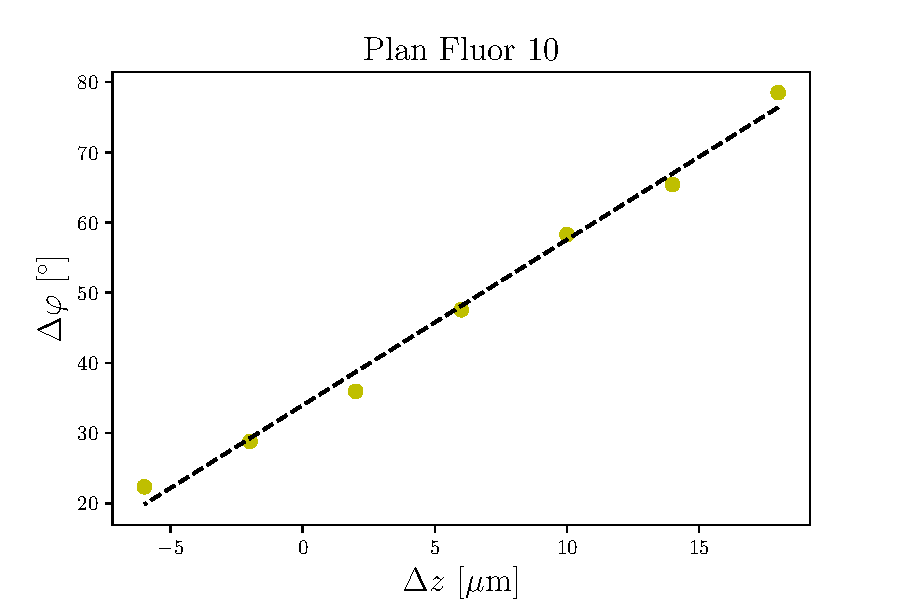
\includegraphics[width=\textwidth]{image/vysledek_10} 
			\caption{} %% aby se ti vysázelo označení obrázku.
		\end{subfigure}
		\begin{subfigure}[h]{0.63\textwidth}
			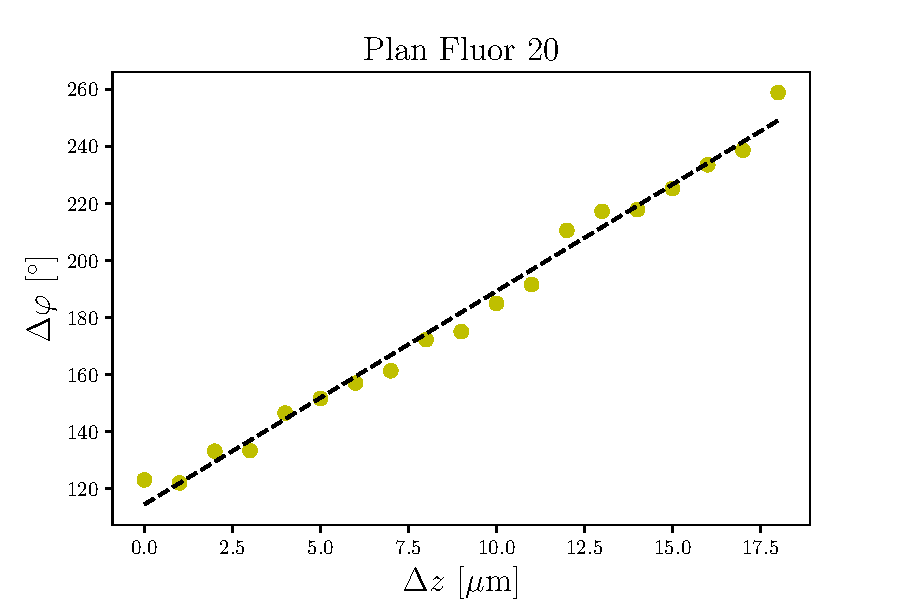
\includegraphics[width=\textwidth]{image/vysledek_20}
			\caption{}
		\end{subfigure}
		\caption[Graf závislosti rotace DH PSF $\Delta\varphi$ na defokusaci objektivu $\Delta z$.]{Graf závislosti rotace DH PSF $\Delta\varphi$ na defokusaci objektivu $\Delta z$, (a) při použití objektivu Plan Fluor 10, (b) při použití objektivu Plan Fluor 20. Měřená data (žluté body) jsou lineárně proloženy (přerušovaná přímka). }
		\label{fig:rotace_grafy}
	\end{figure}
	
		Pokud bys měl více podobrázků přichází do hry balíček \texttt{subcaption}. Pomocí něj lze vysázet i podobrázky. U podobrázků se popisek píše pouze jeden, dolů. Je v tomto připadě vhodné použít navíc hranaté závorky, do nichž se napíše kratší popisek, který se následně ukáže v seznamu obrázků.
	
	Všimni si, že obrázky jsou naschvál široké. Je to proto, aby byly dobře čitelné. Také si všimni popisku grafů. Ačkoli nejspíš netušíš co je to DH PSF či defokusace objektivu mělo by ti být jasné, že je důležité přesně graf popsat. To znamená co je na vodorovné ose, co je na svislé ose. V jakých jednotkách veličiny jsou. Které body co znamenají, která křivka má jaký význam. Napsat samotné \uv{$\Delta \varphi$} je málo, vždy raději připoměň, co daná značka znamená.
	

	
	\subsection{Literatura}
	
	V \LaTeX{}u lze dělat seznam literatury dvěma způsoby. V této šabloně jsem použil ten, kdy se seznam literatury píše přímo do práce. Pro jeho vygenerování doporučuji použít některý z generátarů, jako jsou například Citace PRO \cite{citacePRO}. Pomocí citací lze vygenerovat přímo dokument, který se pak už jen překopíruje do textu a člověk nemusí nic zvýrazňovat. Dále lze využít Bibtex, který rozhodně do budoucna hodlám zaimplementovat do šablony, avšak jeho použití nemusí být tak přátelské k začátečníkům.
	
	Pokud bys chtěl odkazovat na vícero zdrojů stačí je napsat vedle sebe oddělené čárkou \cite{LaTeXprirucka, citacePRO, Born2019}. Případně můžu odkaz na konkrétní stránku dát do hranatých závorek, viz \cite[str.~1]{Born2019}
	
	\subsection{Programový kód}
	Pro vložení programového kódu do dokumentu LaTeX s možností zvýraznění syntaxe můžete použít balíček \texttt{listings}. Tento balíček nabízí široké možnosti pro formátování kódu, včetně zvýraznění syntaxe pro různé programovací jazyky.
	
	Nejprve je třeba do preambule LaTeX dokumentu přidat \texttt{\\usepackage{listings}} a nastavit příslušné parametry. Příklad nastavení pro jazyk Python by mohl vypadat takto:
	


\begin{lstlisting}[style=JavaScript, title={Kód}, caption={Ukázka JS kódu}]
	// JavaScript code here
	function helloWorld() {
		console.log("Hello, world!");
	}
\end{lstlisting}	
	
\begin{lstlisting}[style=ES6, caption={ES6 (ECMAScript-2015) Listing}]
	/* eslint-env es6 */
	/* eslint-disable no-unused-vars */
	
	import Axios from 'axios'
	import { BASE_URL } from './utils/api'
	import { getAPIToken } from './utils/helpers'
	
	export default class User {
		constructor () {
			this.id = null
			this.username = null
			this.email = ''
			this.isActive = false
			this.lastLogin = ''  // ISO 8601 formatted timestamp.
			this.lastPWChange = ''  // ISO 8601 formatted timestamp.
		}
	}
	
	const getUserProfile = async (id) => {
		let user = new User()
		await Axios.get(
		`${BASE_URL}/users/${id}`,
		{
			headers: {
				'Authorization': `Token ${getAPIToken()}`,
			}
		}
		).then{response => {
				// ...
			}).catch(error => {
				// ...
			})
		}
\end{lstlisting}	
	
	\section[Pokročilejší tipy]{Pokročilejší tipy, které se mohou hodit}
	
	\subsection{Rovnice}
	
	Sazba matematiky je věda sama o sobě. Ačkoli Word prošel obrovskou změnou a je v~tomto mnohem lepší, tak \LaTeX je pro to přímo (ještě jsem neviděl matematika, co by používal Word). Spolu s balíčky \texttt{amsmath} a \texttt{amsfonts} snad neexistuje nic, co by se používalo a \LaTeX by to nezvládl. Ať už jde o základní věci jako řecká písmenka -- $\alpha, \beta, \gamma, \dots$ -- integrály -- $\int_{l_i}^{l_f} \tau \dif l $ -- až třeba po speciální písmena -- $\mathscr{F}: \mathbb{R}^n \to \mathbb{R}^m$. Pro případ, že bys potřeboval nějaké speciální integrály, je tu balíček \texttt{esint}, pomocí něj můžeš napsat třeba
	$$ \oiint_{S(V)} \vec{E} \cdot \dif \vec{S} = \iiint_{V} \left(\vec{\nabla} \cdot \vec{E}\right) \dif V .$$
	
	Jak můžeš vidět tak rovnice lze psát jednak do textu a nebo pokud se jedná o nějakou důležitou nebo rozsáhlejší rovnici tak na samostatný řádek. Pokud je rovnice opravdu důležitá, tak je vhodné ji také číslovat. Pak se na ni můžeš dále odkazovat v textu.
	\begin{equation}
		\vec{F} = m \vec{a}
		\label{eq:newton2}
	\end{equation}
	\dots Například podle druhého Newtonova zákona, rovnice (\ref{eq:newton2}) \dots Zároveň je vždy nutné vysvětlit co která veličina znamená. V tomto případě bych napsal, že v druhém Newtonově zákoně vektor síly $\vec F$ odpovídá součinu hmotnosti tělesa $m$ a jeho zrychlení $\vec a$. 
	
	Věřím, že se sazbou matematiky ti pomůže tvůj školitel, případně mi můžeš napsat (mail je v úvodu). Jednotlivé funkcionality spolu se seznamem znaků nalezneš jednak v Ne příliš stručném úvodu~\cite{LaTeXprirucka} nebo na Wikibooks v sekcích \emph{Mathematics} a \emph{Advanced mathematics}~\cite{wikibooksLaTeX}.
	
	
	
	
	\chapter{Když dokončuji práci}
	
	Každou práci je dobré zkontrolovat, aby v ní nebyly pravopisné chyby, nebyla těžkopádně napsaná -- byla čtivá -- a neobsahovala žádný typografický nedostatek. Proto, když práci sepíšeš, nech ji chvilku odležet, třeba týden. Pak si ji po sobě znovu přečti. Hned uvidíš, kolik věcí bys napsal jinak případně kde tě bije do očí jaká chyba. Dej práci přečíst také svému školiteli a případně češtináři. Zajistíš tak, že bude obsahovat méně chyb.
	
	Pak můžeš práci vytisknout a hurá do soutěže.
	
	\chapter*{Závěr}
	
	Věřím, že jsem ti spolu se šablonou poskytl několik tipů, jak napsat práci. Ať už jde o úplné začátky s \LaTeX{}em. Či ukázku toho, co vše s ním zvládneš. Pokud bys měl k šabloně libovolné dotazy, rouhodně se na mě obrať. \LaTeX tvé práci dodá určitou krásu, tak doufám, že ti dodá sebevědomí a uspěješ při souteži. A i kdyby ne vzpomeň si, kolik ses toho musel naučit a hned uvidíš o jaký kus ses posunul.
	
	%% literatura
	\begin{thebibliography}{99}
		\bibitem{sablonaSOC} DOKULIL Jakub. \textit{Šablona pro psaní SOČ v programu \LaTeX} [Online]. Brno, 2020 [cit. 2020-08-24]. Dostupné z: \url{https://github.com/Kubiczek36/SOC_sablona}
		\bibitem{LaTeXprirucka}OETIKER, Tobias, Hubert PARTL, Irene HYNA, Elisabeth SCHEGL, Michal KOČER a Pavel SÝKORA. \textit{Ne příliš stručný úvod do systému LaTeX2e} [online]. 1998 [cit. 2020-08-24]. Dostupné z: \url{https://www.jaroska.cz/elearning/informatika/typografie/lshort2e-cz.pdf}
		\bibitem{wikibooksLaTeX}\textit{Wikibooks: LaTeX} [online]. San Francisco (CA): Wikimedia Foundation, 2001- [cit. 2020-08-24]. Dostupné z: \url{https://en.wikibooks.org/wiki/LaTeX}
		\bibitem{stackExchange} \textit{TeX - LaTeX Stack Exchange} [online]. Stack Exchange, 2020 [cit. 2020-09-01]. Dostupné z: \url{https://tex.stackexchange.com}
		\bibitem{sspuLogo} \textit{Střední škola průmyslová a umělecká Opava} [online]. [cit. 2023-11-11]. Dostupné z: \url{https://www.sspu-opava.cz}
		\bibitem{citacePRO}\textit{Citace PRO} [online]. Citace.com, 2020 [cit. 2020-08-31]. Dostupné z: \url{https://www.citacepro.com}
		\bibitem{Born2019} BORN, Max a Emil WOLF. \textit{Principles of optics: electromagnetic theory of propagation, interference and diffraction of light}. 7th (expanded) edition. Reprinted wirth corrections 2002. 15th printing 2019. Cambridge: Cambridge University Press, 2019. ISBN 978-0-521-64222-4.
	\end{thebibliography}
	
	%% obrázky 
	\listoffigures
	
	%% tabulky
	\listoftables
	
	\appendix %% začínají přílohy
	
	\titleformat{\chapter}[block]{\scshape\bfseries\LARGE}{Příloha \thechapter}{10pt}{\vspace{0pt}}[\vspace{-22pt}] %% nastavení nadpisu u příloh
	
	
	\chapter{%Příloha A 
		Spot diagramy a další }
	
	
\end{document}